\documentclass[a4paper]{article}

%% Language and font encodings
\usepackage[english]{babel}
\usepackage[utf8x]{inputenc}
\usepackage[T1]{fontenc}

%% Page size and margins
\usepackage[a4paper,top=3cm,bottom=2cm,left=3cm,right=3cm,marginparwidth=1.75cm]{geometry}

%% Packages
\usepackage{amsmath}
\usepackage{bm}
\usepackage{graphicx}
\usepackage{algorithm}
\usepackage{float}
\usepackage{caption}
\usepackage{subcaption}
\usepackage{enumerate}
\usepackage[noend]
{algpseudocode}
\setlength{\marginparwidth}{2cm}
\usepackage[colorinlistoftodos]{todonotes}
\usepackage[colorlinks=false, allcolors=blue]{hyperref}
\usepackage{textcomp}

\title{\textbf{CMOS References and Regulators: Homework}}
\author{Chamarthy Madhan Sai Krishna\\2023102030}

\begin{document}

\maketitle

\tableofcontents

\section{Lecture 1}

\subsection{Question 1}
Do the 'DC Analysis' for the following circuits. Plot V vs I $\&$ write expression for the slope. Prove that its a resistance.\\
\begin{figure}
    \centering
    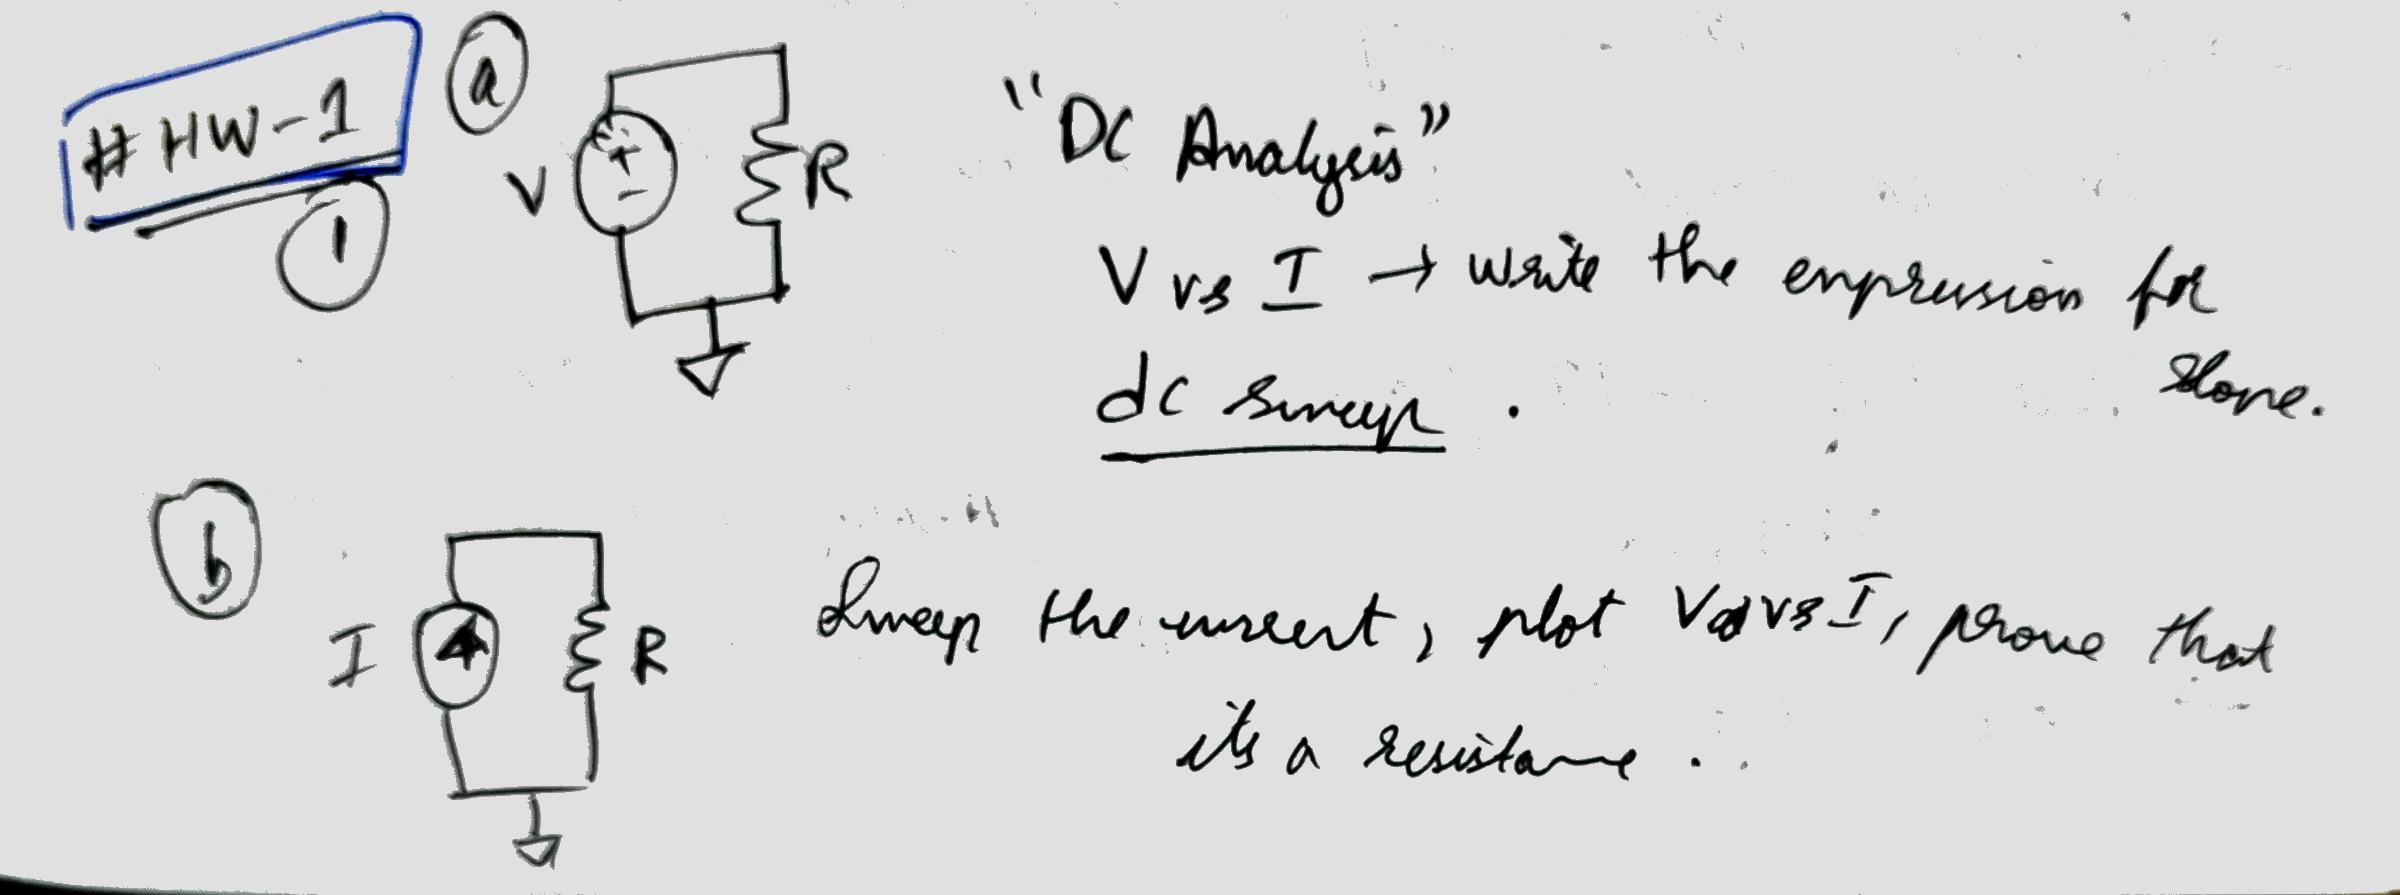
\includegraphics[width=0.8\linewidth]{images/Lec_1_Q_1.jpeg}
    \caption{Lecture 1 - Question 1 - (a) and (b)}
\end{figure}
\textit{Answer: }\\
Left graph shows the I - V characteristics of the device. Clearly, $I \propto V$. The right graph shows the expression for the slope. \\
Plot for (a) : Using a Voltage source \\
Plot for (b) : Using a Current source

\begin{figure}[ht]
    \centering
    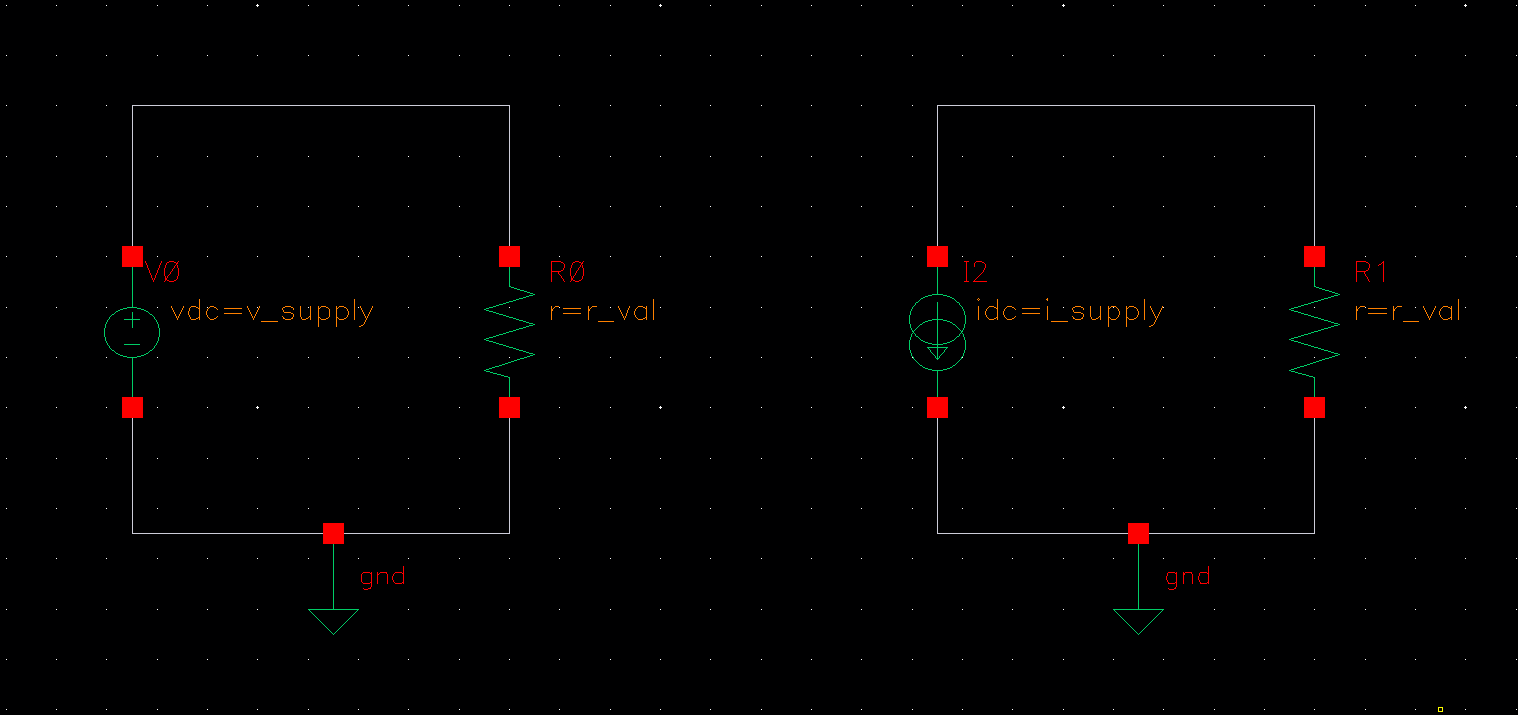
\includegraphics[width=1\linewidth]{images/Lec_1_Q_1_testbench.png}
    \caption{Testbench for (a) and (b)}
\end{figure}

\begin{figure}
    \centering
    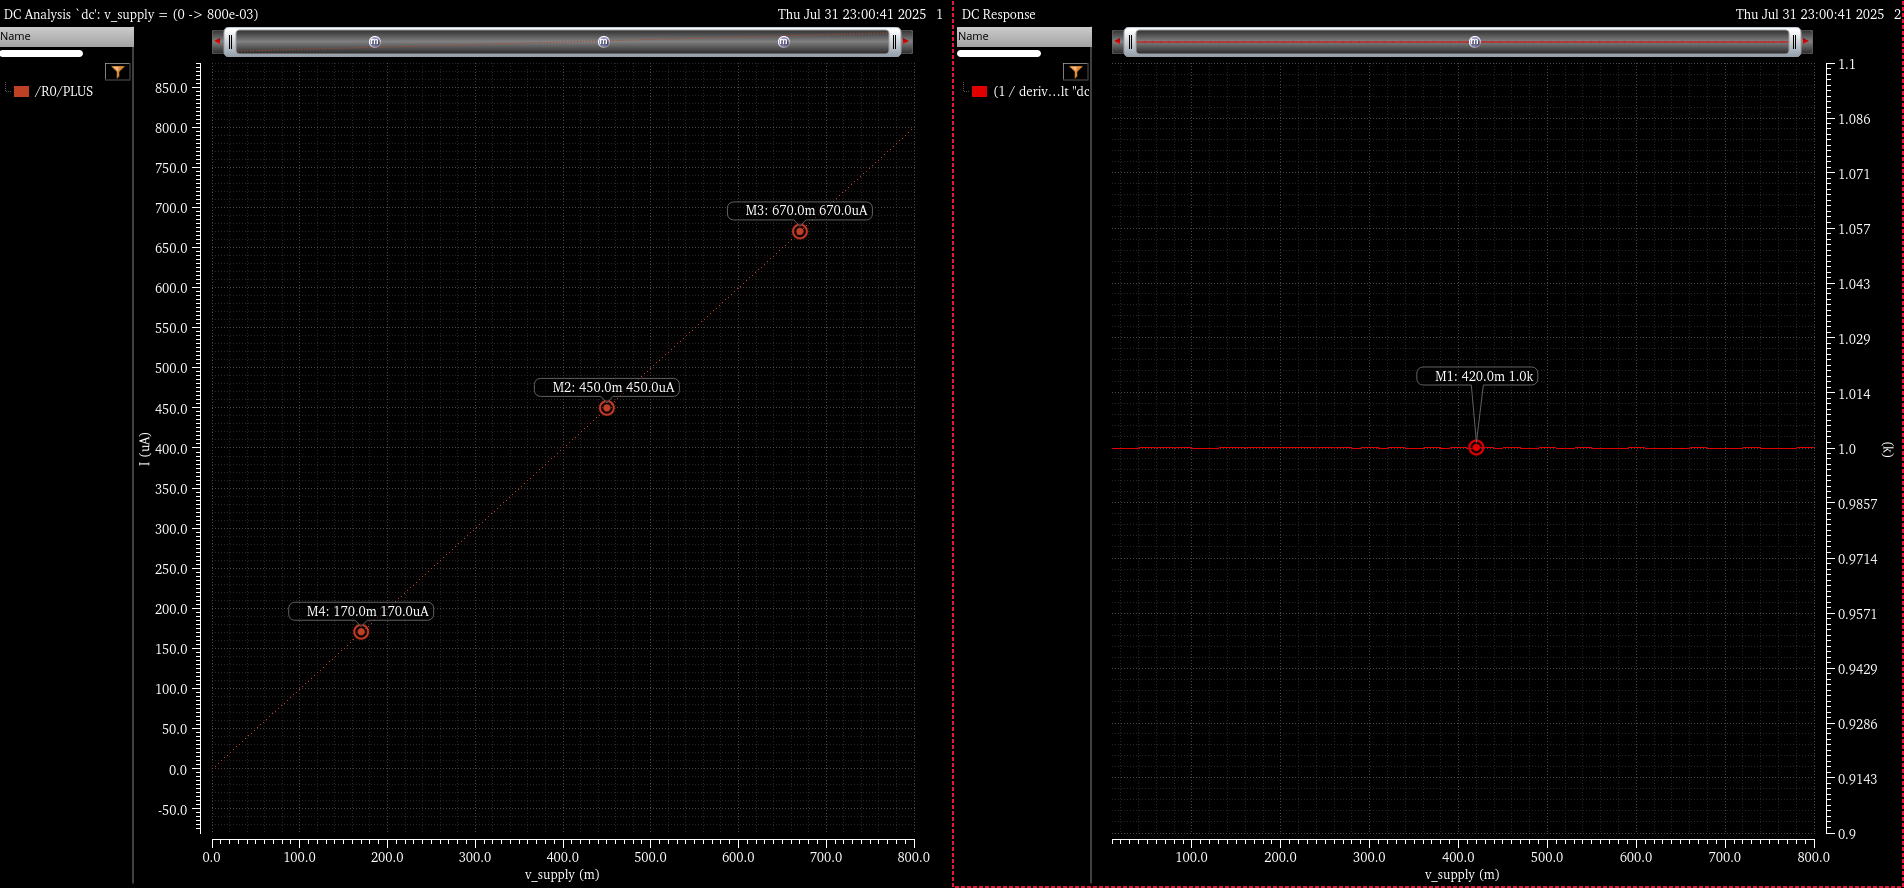
\includegraphics[width=1\linewidth]{images/Lec_1_Q_1_a_plot.png}
    \caption{Plot for (a)}
\end{figure}

\begin{figure}
    \centering
    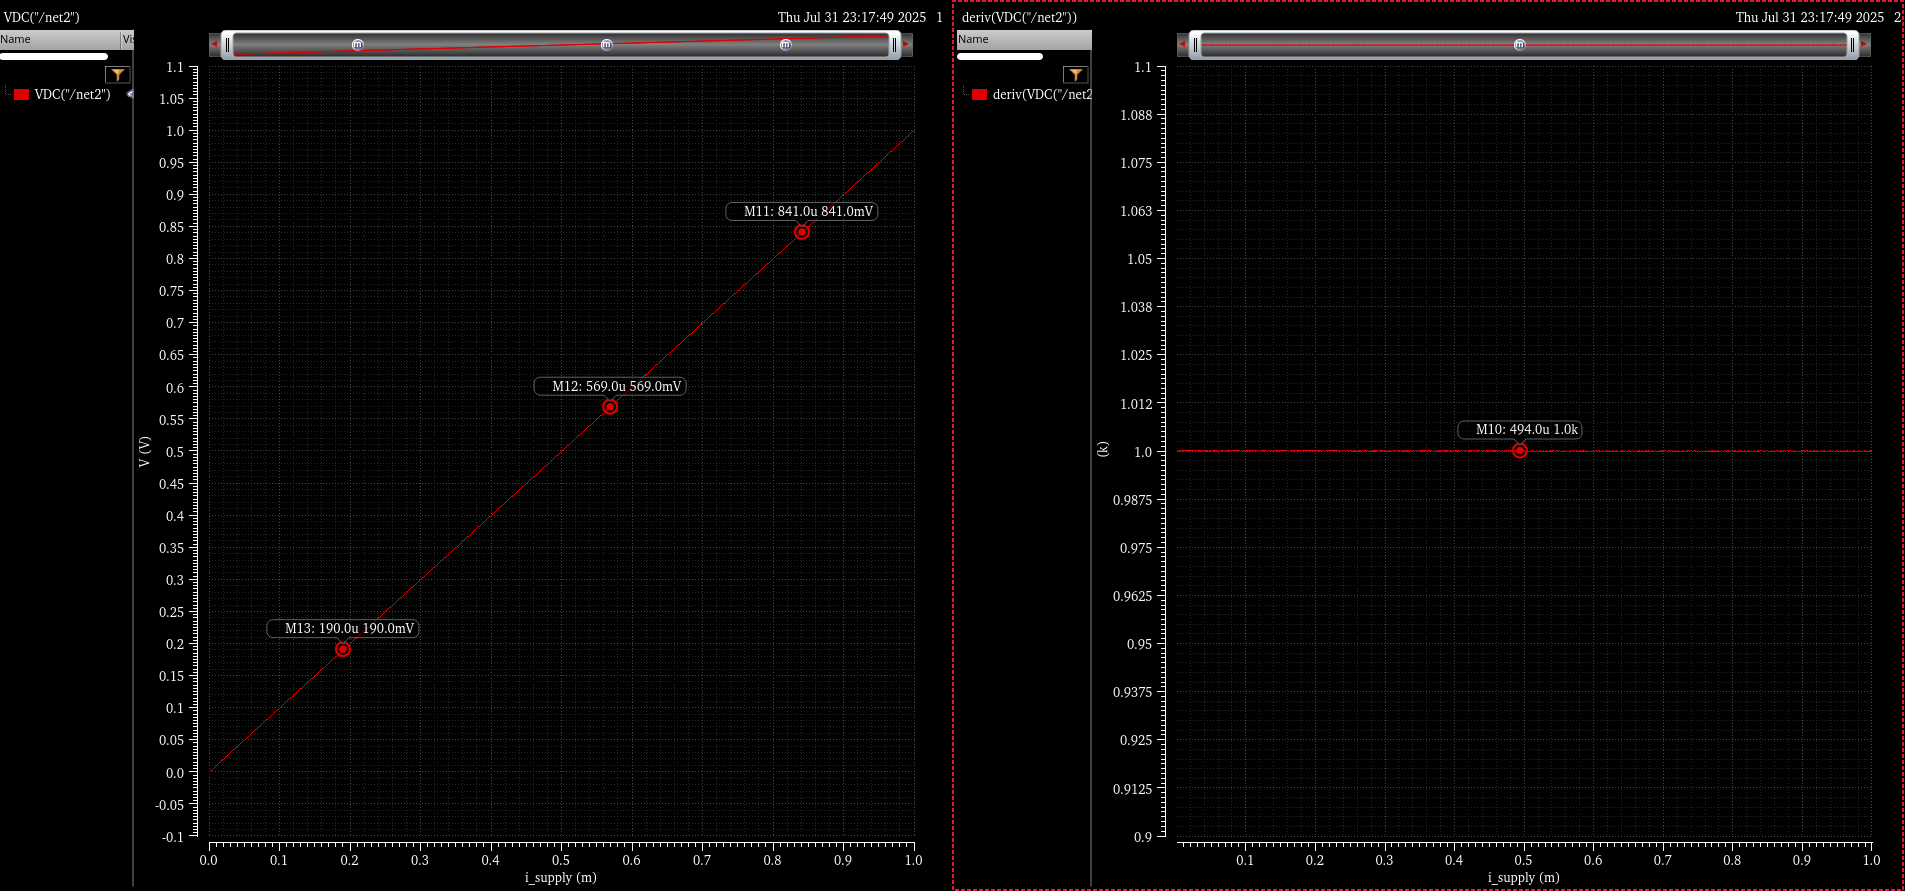
\includegraphics[width=1\linewidth]{images/Lec_1_Q_1_b_plot.png}
    \caption{Plot for (b)}
\end{figure}

\subsection{Question 2}
Design a capacitance amplifier using controlled sources.\\
\begin{figure}
    \centering
    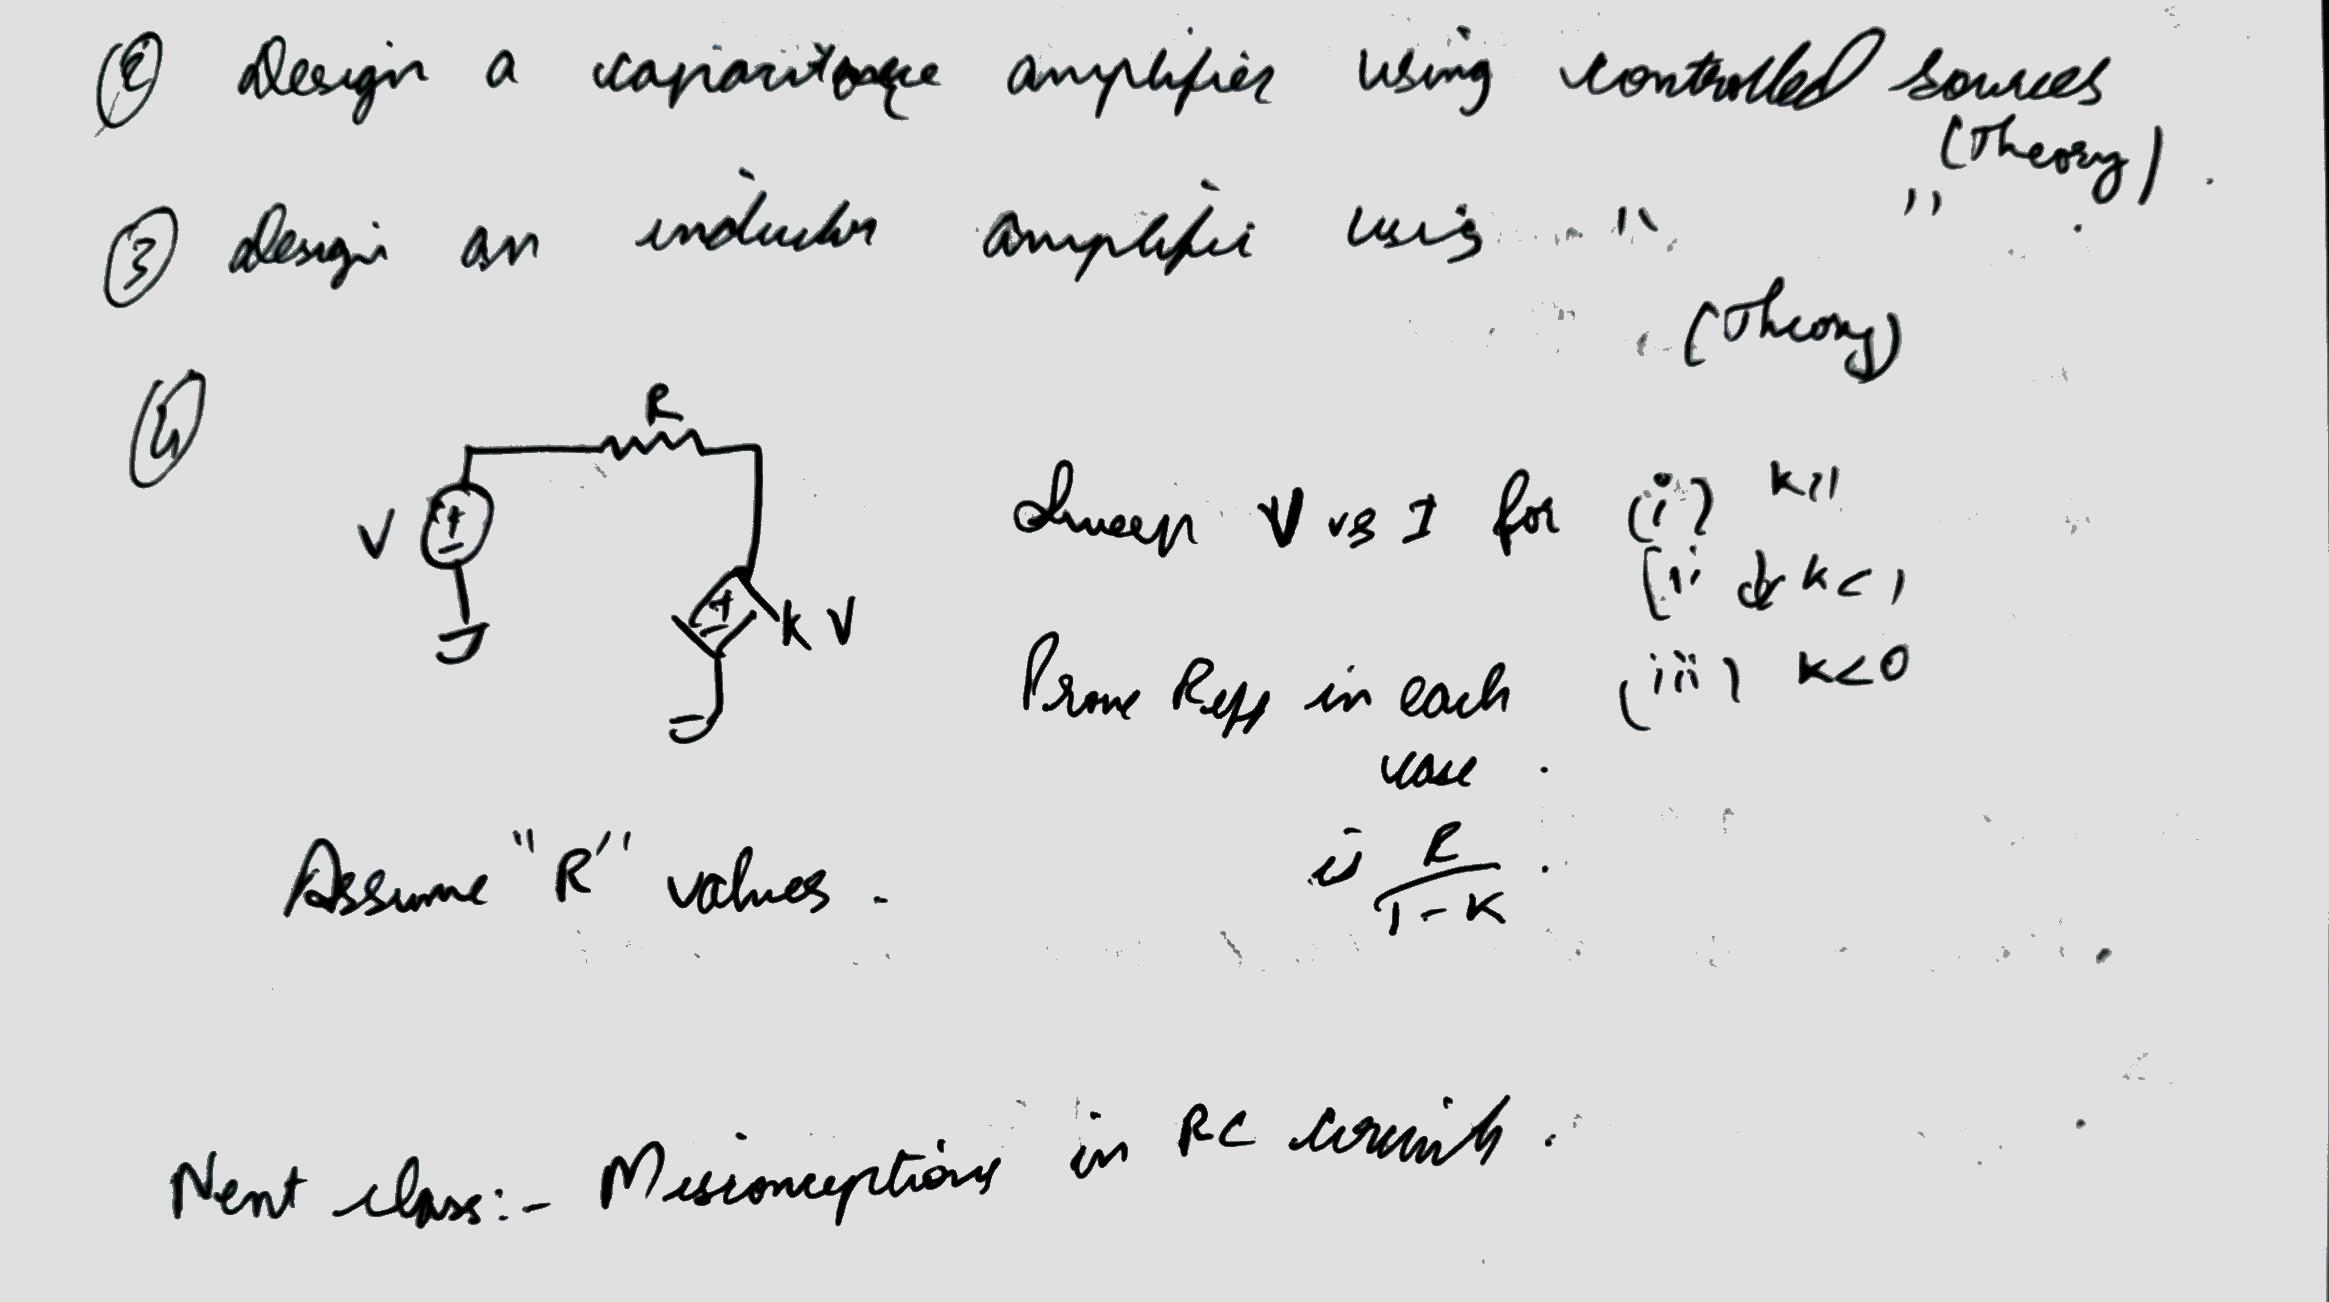
\includegraphics[width=0.8\linewidth]{images/Lec_1_Q_2_3_4.jpeg}
    \caption{Lecture 1 - Question 2, 3, 4}
\end{figure}
\textit{Answer: }\\

\subsection{Question 3}
Design a capacitance amplifier using controlled sources.\\

\textit{Answer: }\\

\subsection{Question 4}
Sweep V vs I for (i) $k>1$ (ii) $0<k<1$ (iii) $K<0$ Prove $R_{eff}$ in each case is $\frac{R}{1-k}$.\\
\textit{Answer: }\\

\section{Lecture 2}
\subsection{Question 1}
find the effective output resistance at $V_{out}$ i.e., $R_{out} = ?$ \\
\begin{figure}
    \centering
    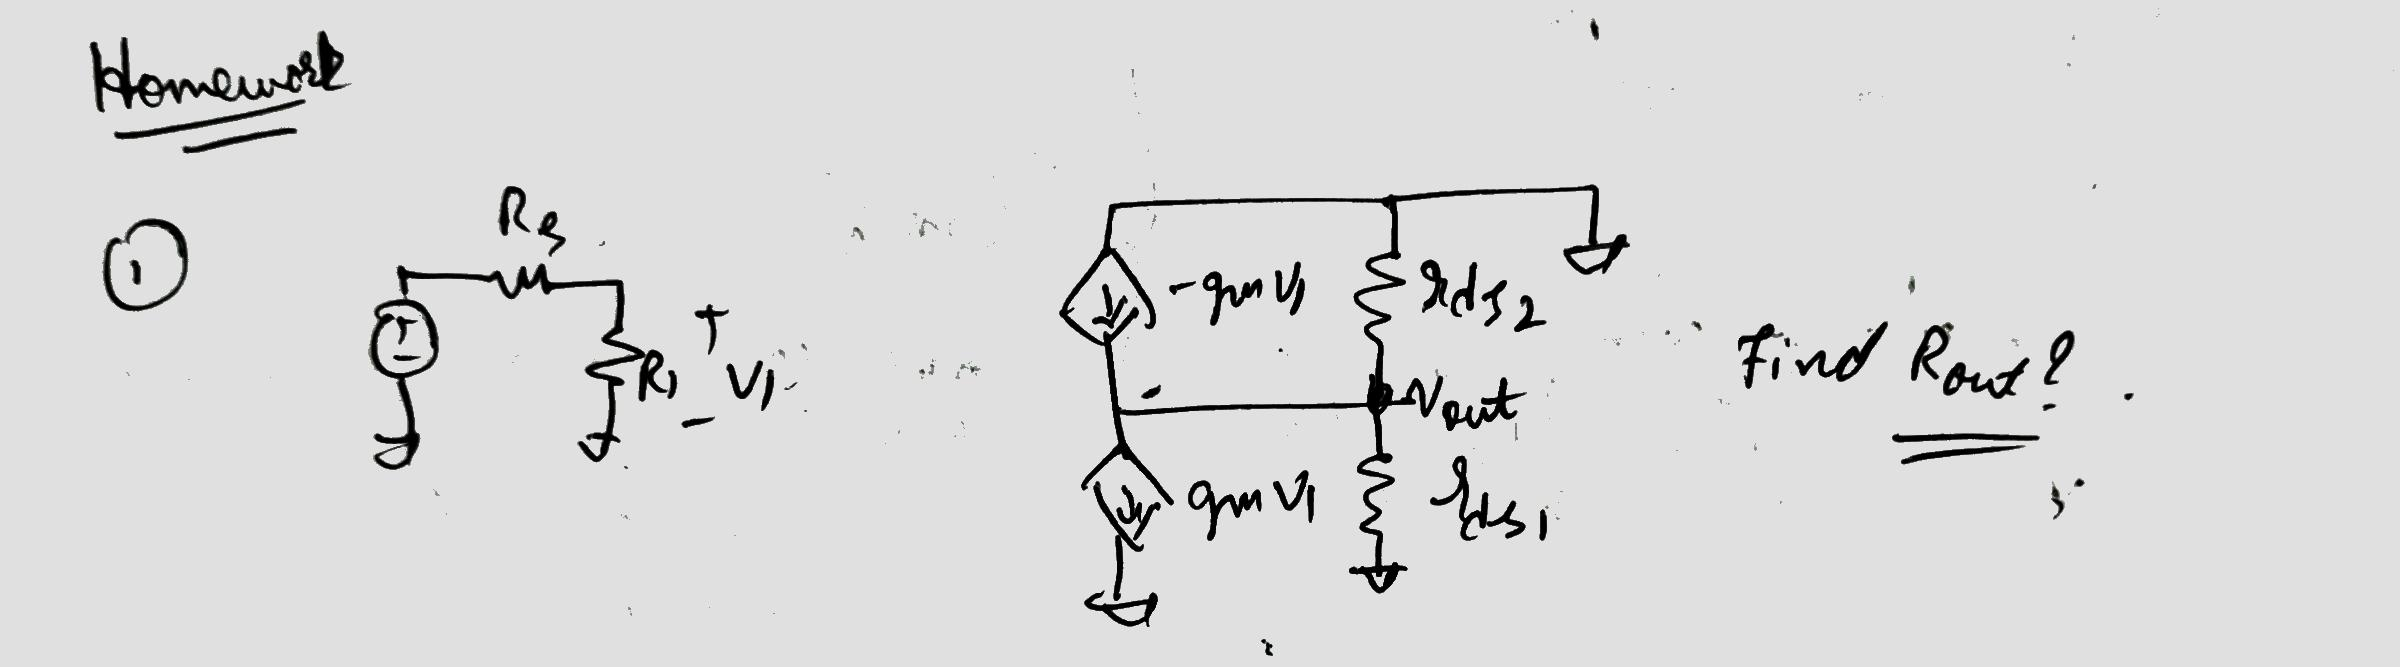
\includegraphics[width=0.8\linewidth]{images/Lec_2_Q_1.jpeg}
    \caption{Lecture 2 - Question 1}
\end{figure}
\textit{Answer:}\\
When we nullify the V1, the vccs vanish and the effective output resistance at vout node is $R_{out} = r_{ds_1} || r_{ds_2}$. 
Proved this using the plot with values.

\begin{figure}
    \centering
    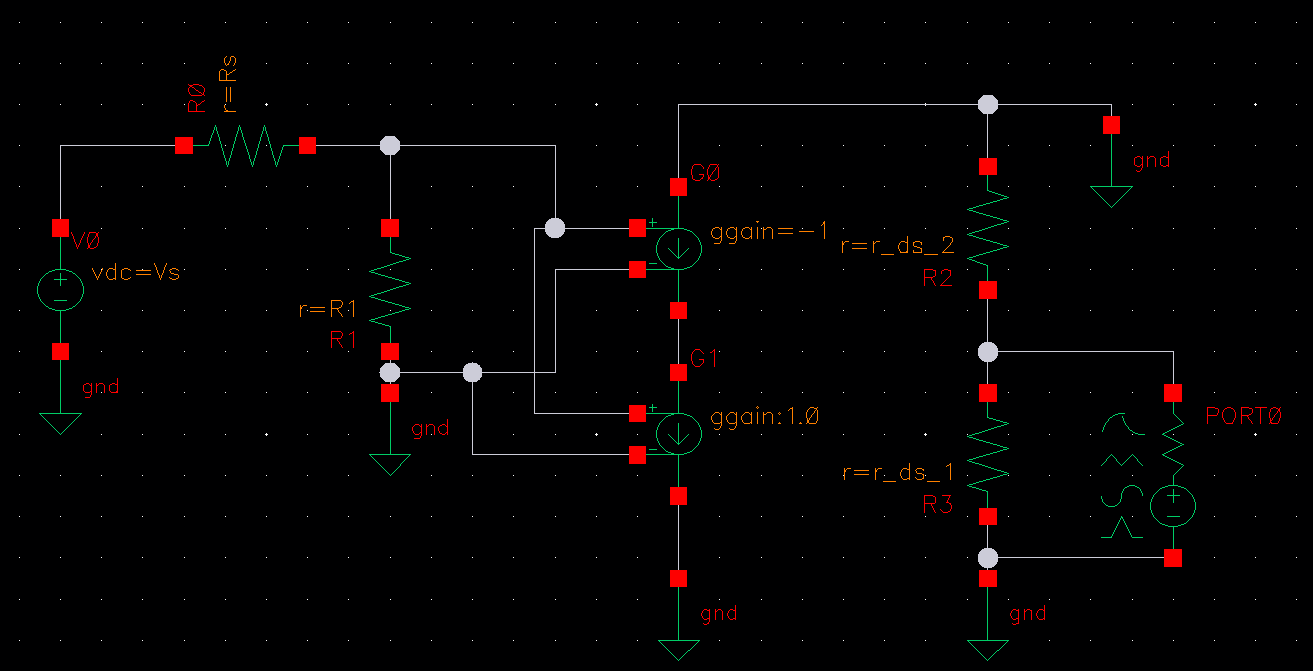
\includegraphics[width=1\linewidth]{images/Lec_2_Q_1_testbench.png}
    \caption{Testbench}
\end{figure}

\subsection{Question 2}
Plot $V_{out}$ vs time in Cadence. Prove Theory. \\
\begin{figure}
    \centering
    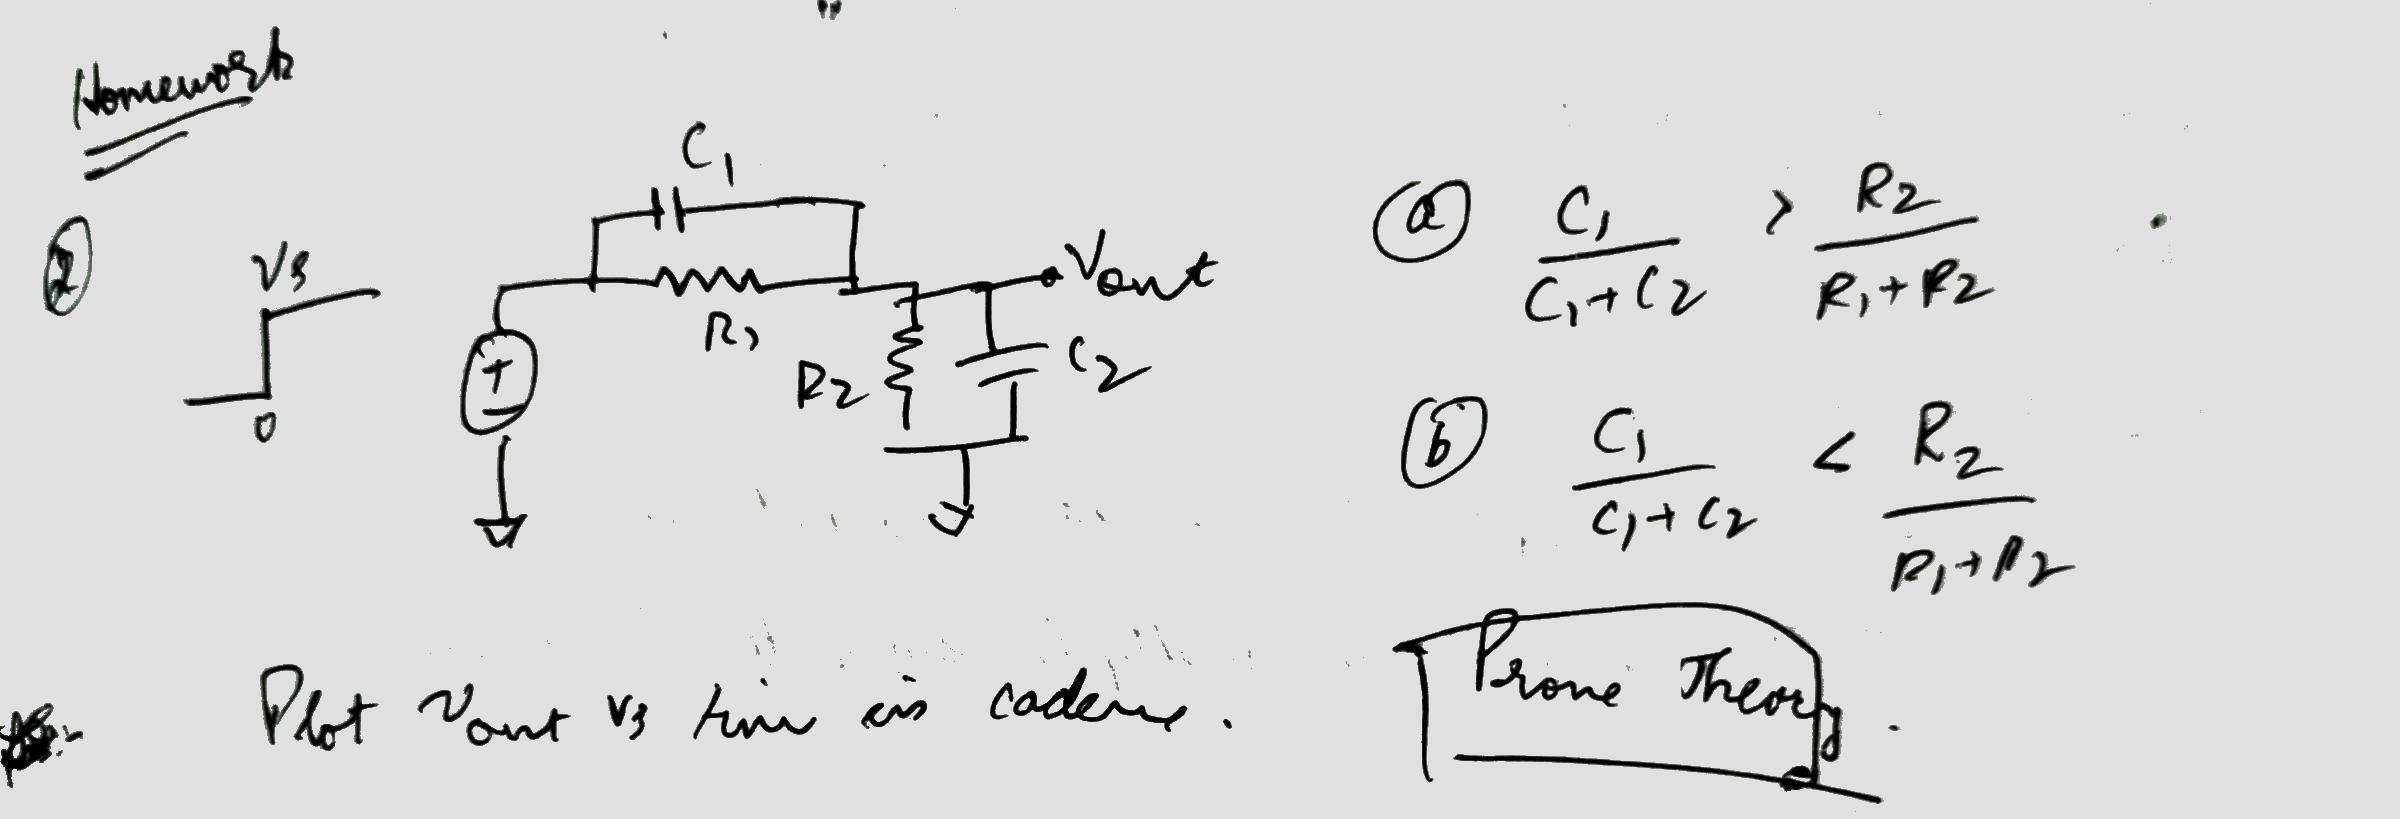
\includegraphics[width=0.8\linewidth]{images/Lec_2_Q_2.jpeg}
    \caption{Lecture 2 - Question 2}
\end{figure}
\textit{Answer:}\\
Copy this from the notes\\
Proved this using theory and from the simulations  by finding the output voltage after 1 time constant.

\begin{figure}
    \centering
    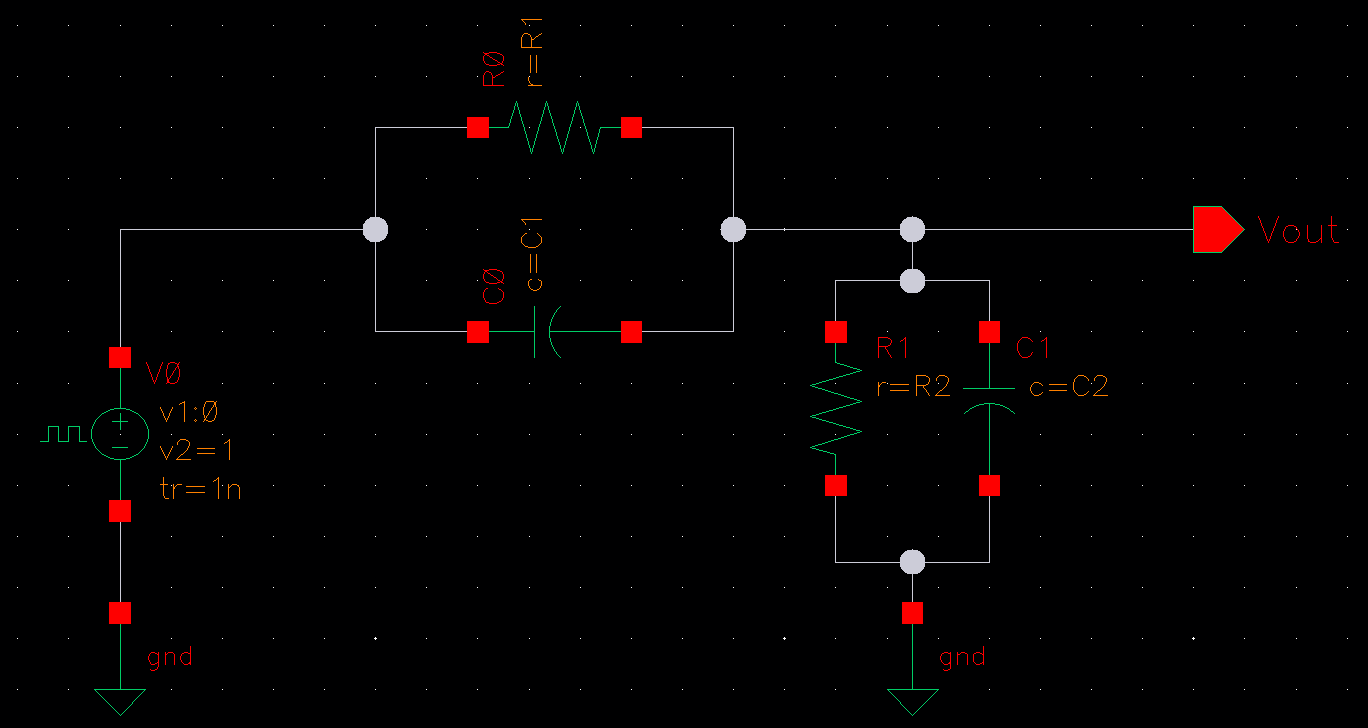
\includegraphics[width=1\linewidth]{images/Lec_2_Q_2_testbench.png}
    \caption{Question 2 Testbench}
\end{figure}

\begin{figure}
    \centering
    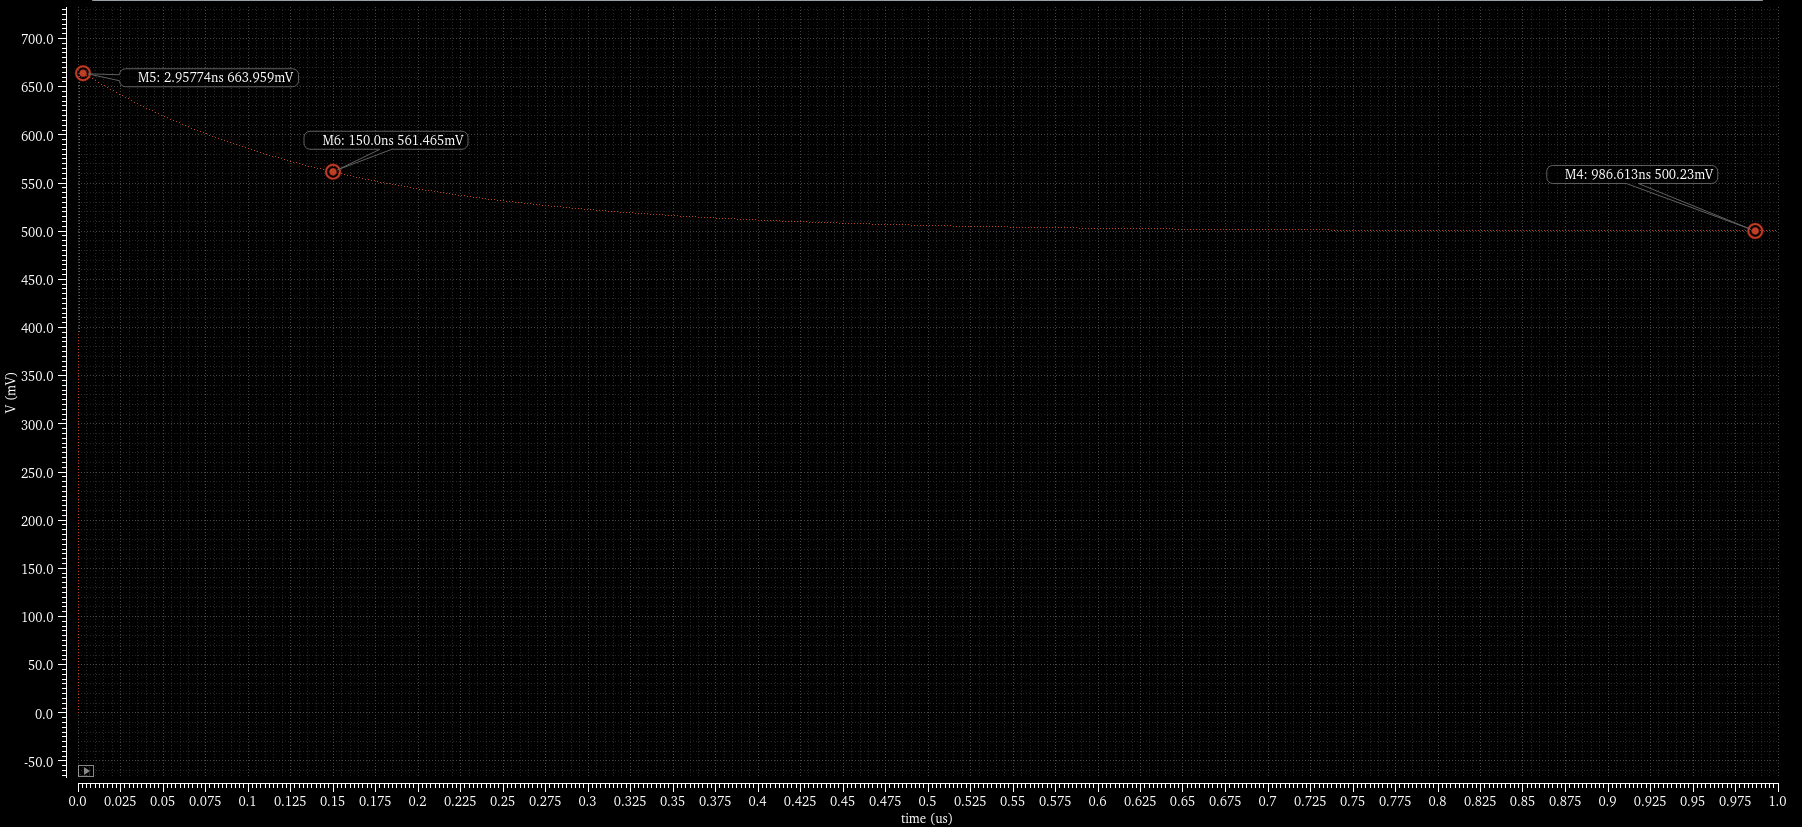
\includegraphics[width=1\linewidth]{images/Lec_2_Q_2_a.png}
    \caption{Part (a)}
\end{figure}

\begin{figure}
    \centering
    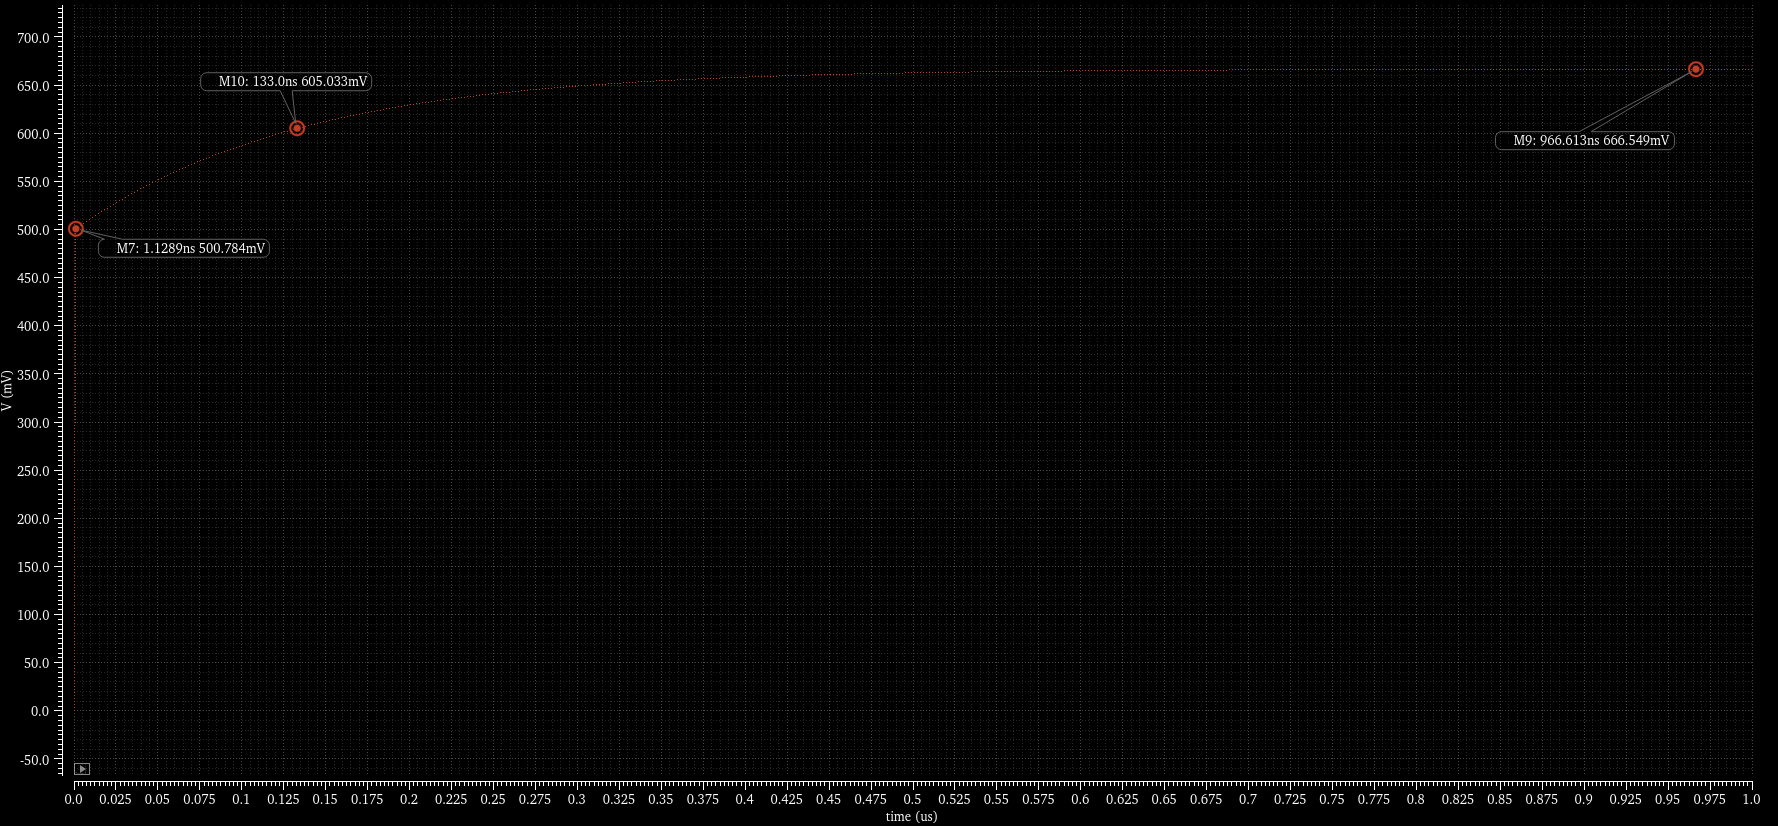
\includegraphics[width=1\linewidth]{images/Lec_2_Q_2_b.png}
    \caption{Part (b)}
\end{figure}

\section{Lecture 3}
\subsection{Question 1}
Plot $V_{out}$ vs $time$ and $I_{out}$ vs $time$
\begin{itemize}
    \item 
    \item 
    \item 
\end{itemize}
\begin{figure}
    \centering
    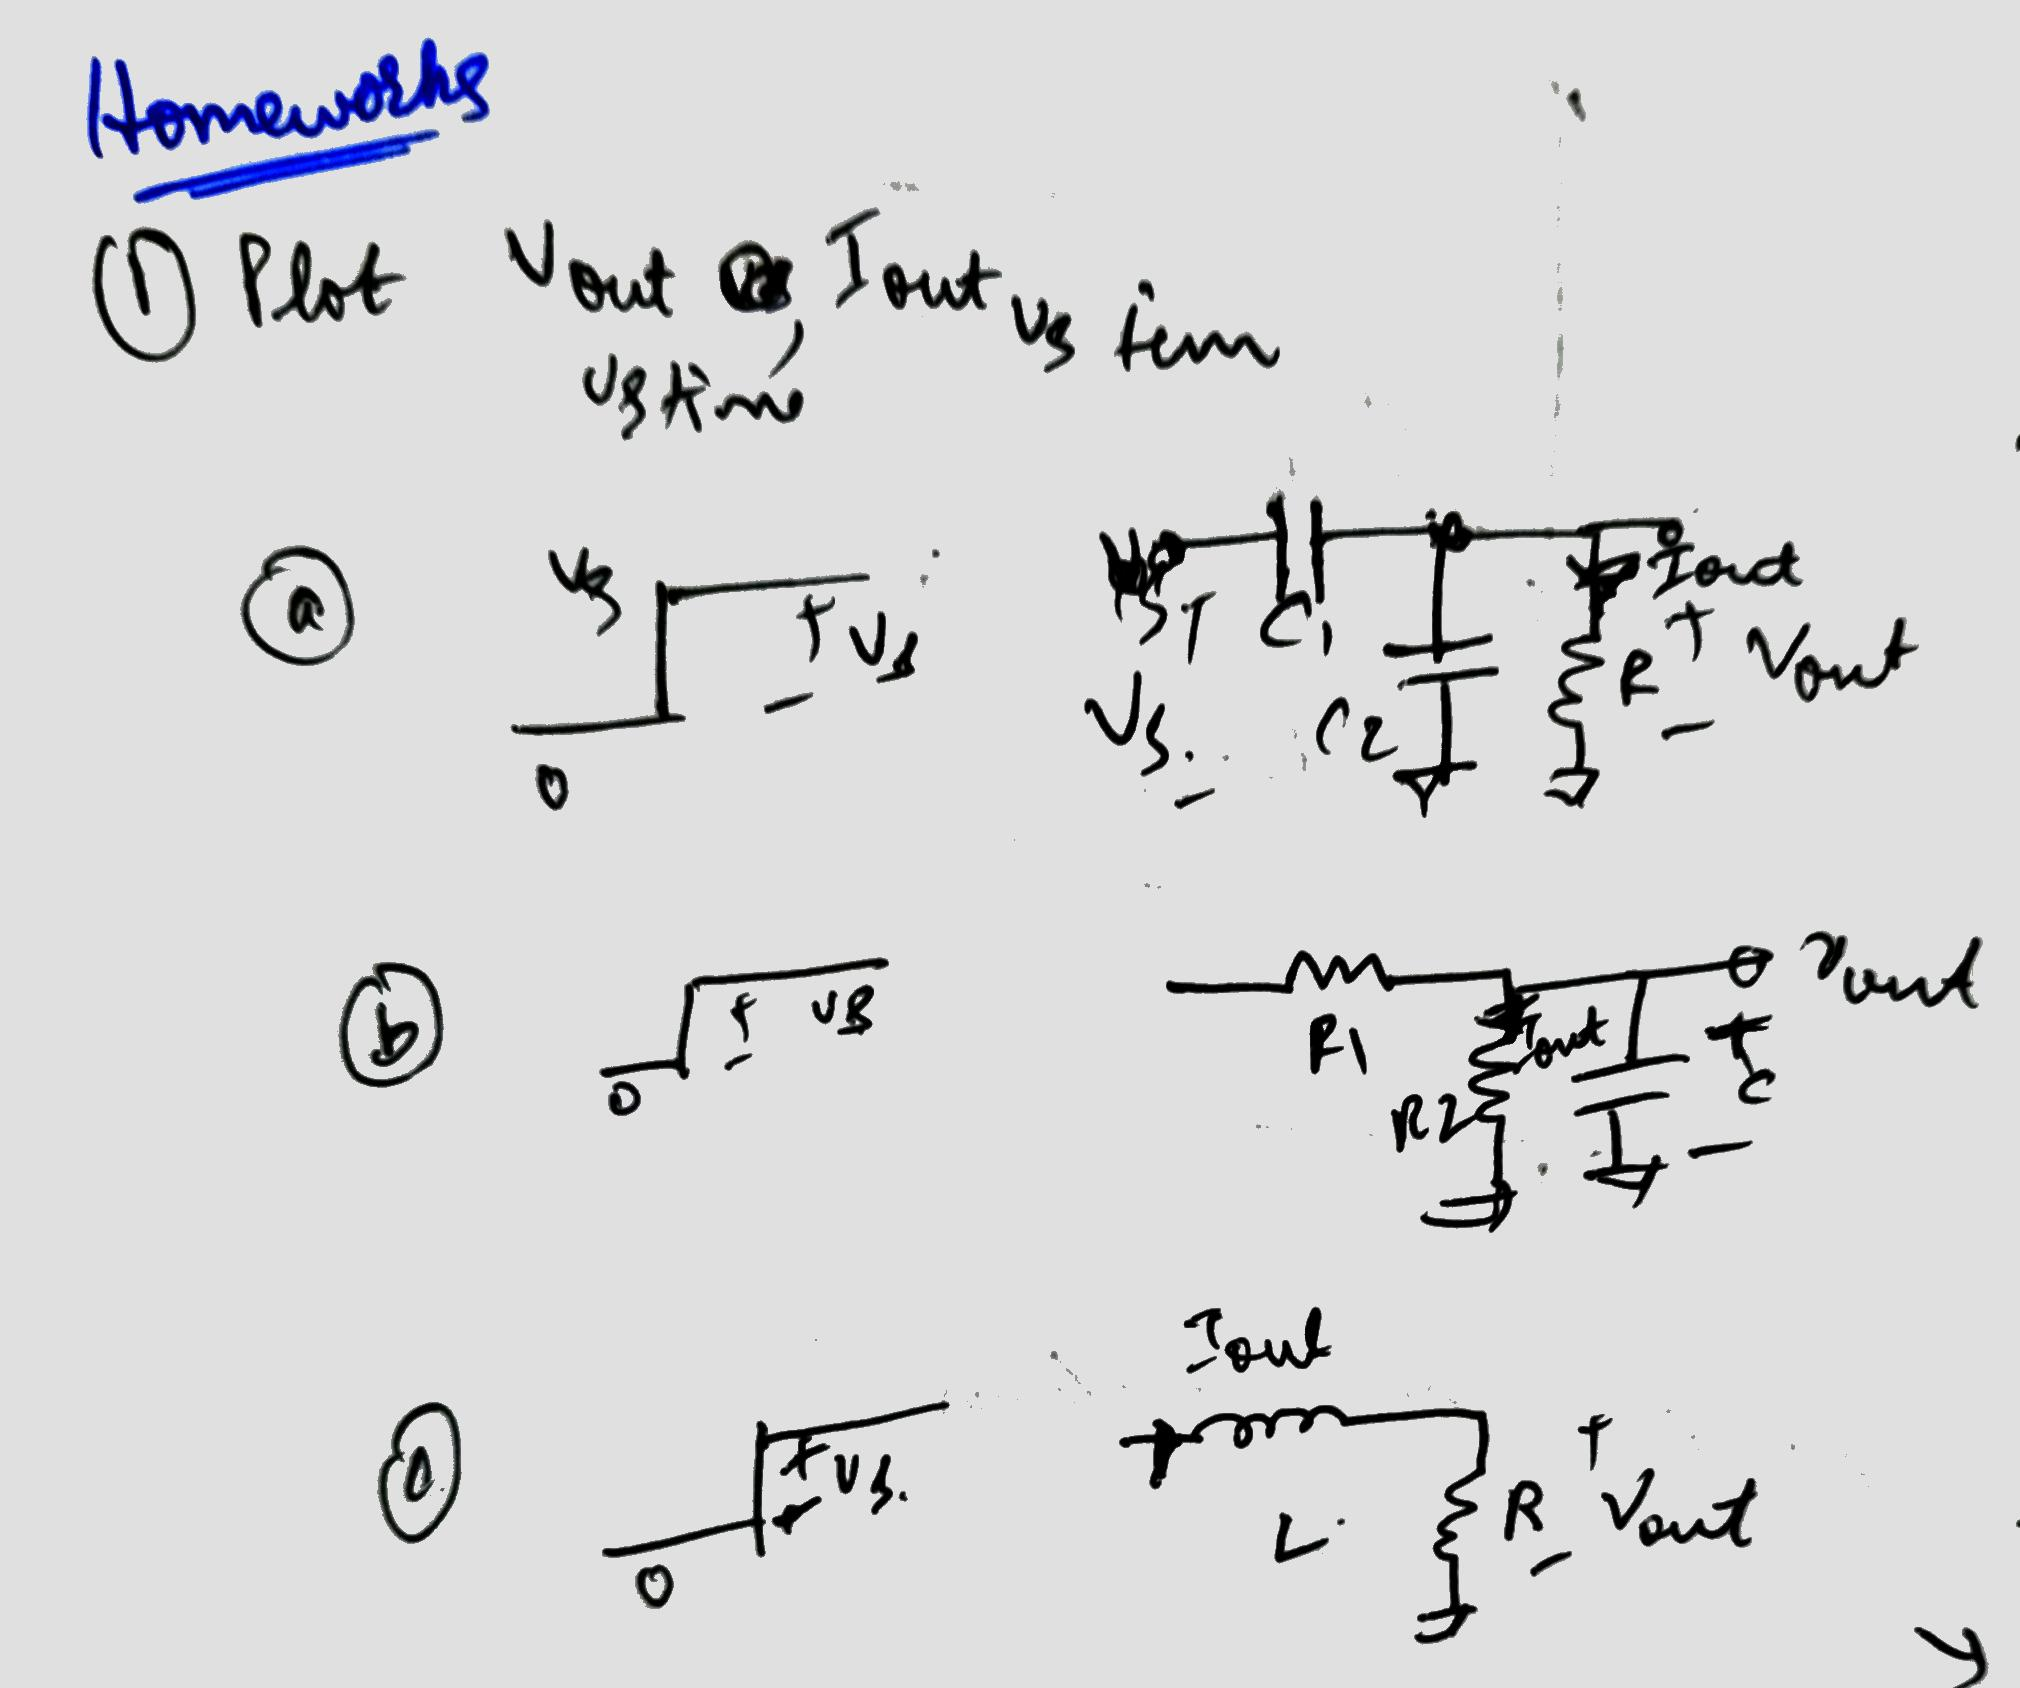
\includegraphics[width=0.8\linewidth]{images/Lec_3_Q_1.jpeg}
    \caption{Lecture 3 - Question 1}
\end{figure}
\subsection{Question 2}
Plot $V_{out}$ vs $time$ (a) $D = 10\%$ (b) $D = 90\%$ (i) $T = 0.1RC$ (ii) $T = 10RC$ where $D = \frac{T_{ON}}{T}$
\begin{figure}
    \centering
    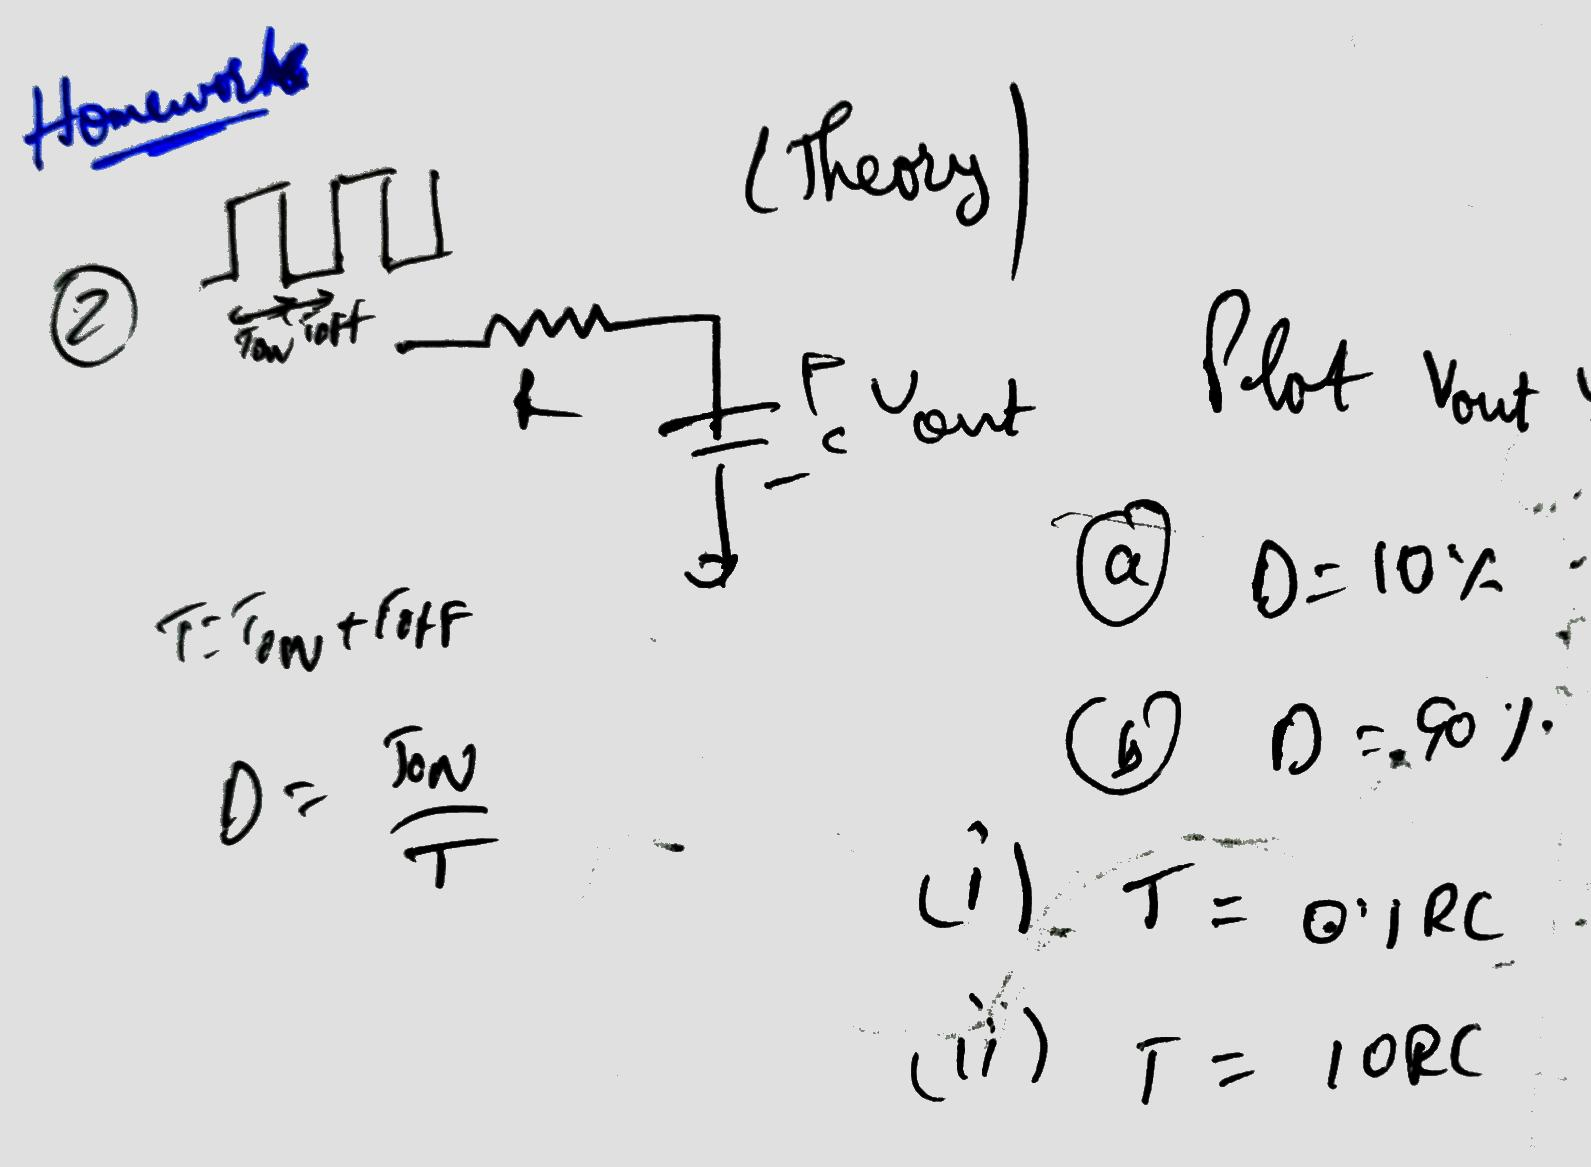
\includegraphics[width=0.8\linewidth]{images/Lec_3_Q_2.jpeg}
    \caption{Lecture 3 - Question 2}
\end{figure}
\subsection{Question 3}
Draw Bode plot for $H(s) = \frac{(s - z_1)(s+z_2)}{(s+P_1)(s+P_2)(s+P_3)}$ where (i) $z_2 << p_1 << p_2 << p_3 << z_1$ (ii) $p_3 << p_2 << p_1 << z_1 << z_2$
\begin{figure}
    \centering
    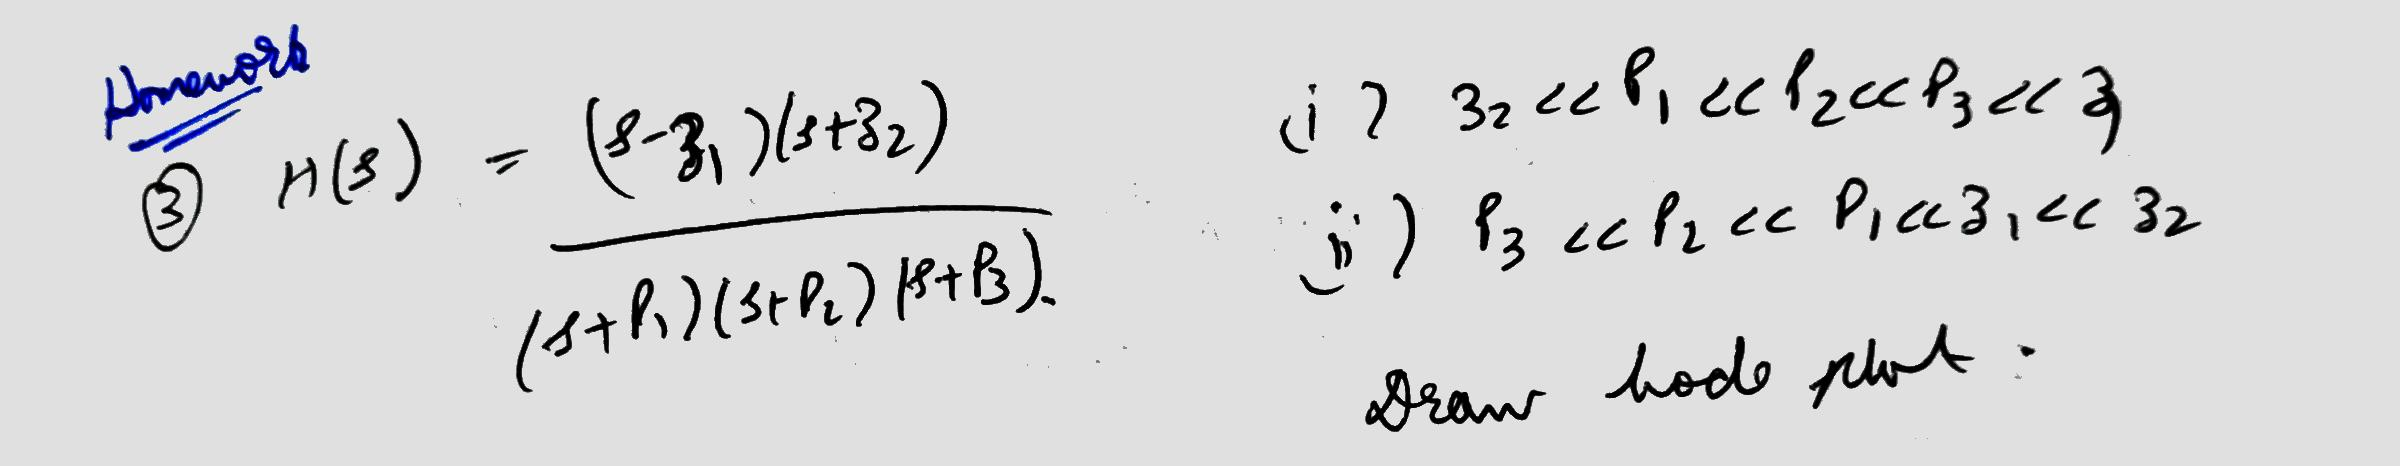
\includegraphics[width=0.8\linewidth]{images/Lec_3_Q_3.jpeg}
    \caption{Lecture 3 - Question 3}
\end{figure}

\section{Lecture 4}
\subsection{Question 1}
Design a non-inverting schimdt trigger using opamp based circuits.
\begin{figure}
    \centering
    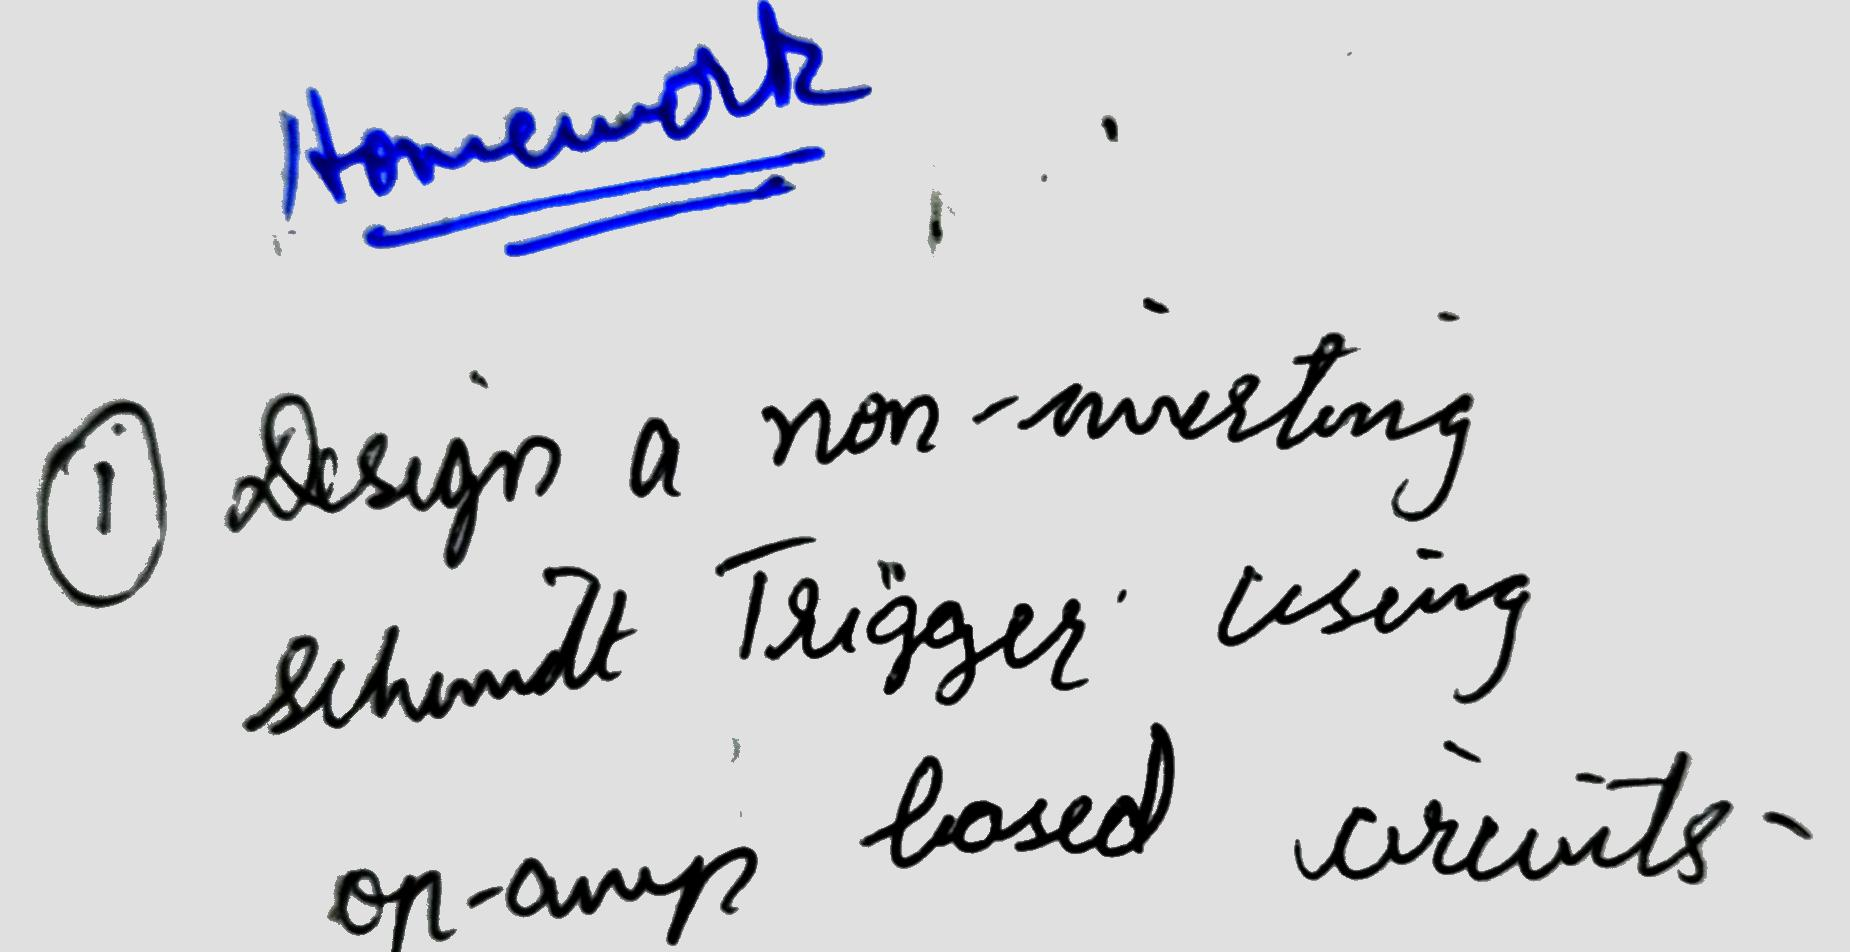
\includegraphics[width=0.8\linewidth]{images/Lec_4_Q_1.jpeg}
    \caption{Lecture 4 - Question 1}
\end{figure}
\subsection{Question 2}
Find the expression for Closed loop Unity gain bandwidth.
\begin{figure}
    \centering
    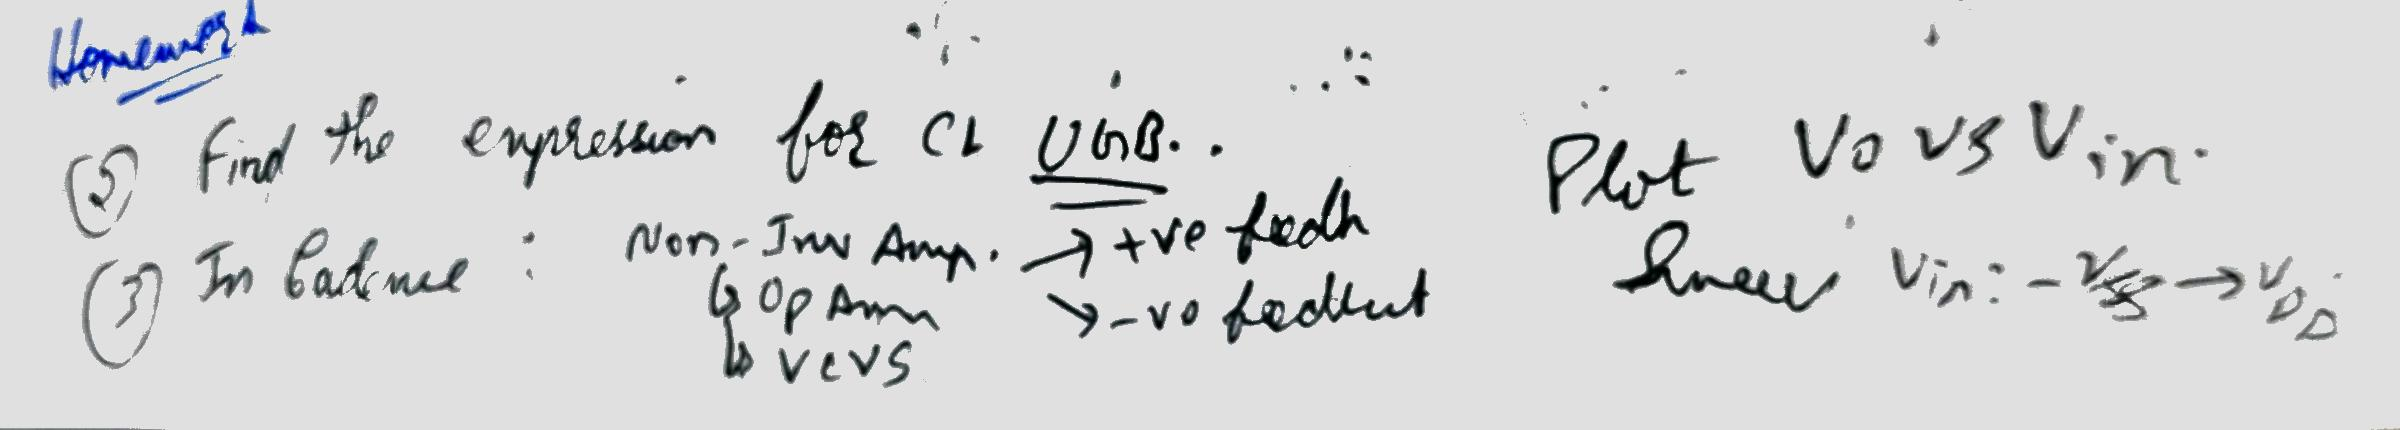
\includegraphics[width=0.8\linewidth]{images/Lec_4_Q_2_3.jpeg}
    \caption{Lecture 4 - Question 2,3}
\end{figure}
\subsection{Question 3}
In cadence, Plot $V_o$ vs $V_{in}$ (Sweep $V_{in}$ from $-V_{ss}$ to $V_{DD}$) for non-inverting amplifier using Opamp and VCVS for both positive and -ve feedback.
\section{Lecture 5}
\subsection{Question 1}
In Cadence, Bode Plot for 
\begin{enumerate}
    \item A = 100, check $V_x$ (offset) [DC]
    \item A = 1000, check $V_x$ (offset) [DC]
    \item UGB = 1MHz, Gain = 1000, Design $G_m$, $R_{out}$, $R_{1}$, $R_{2}$, $C$, $V_{Ref} = 0.6V$, $V_{out} = 1.2V$
\end{enumerate}
\begin{figure}
    \centering
    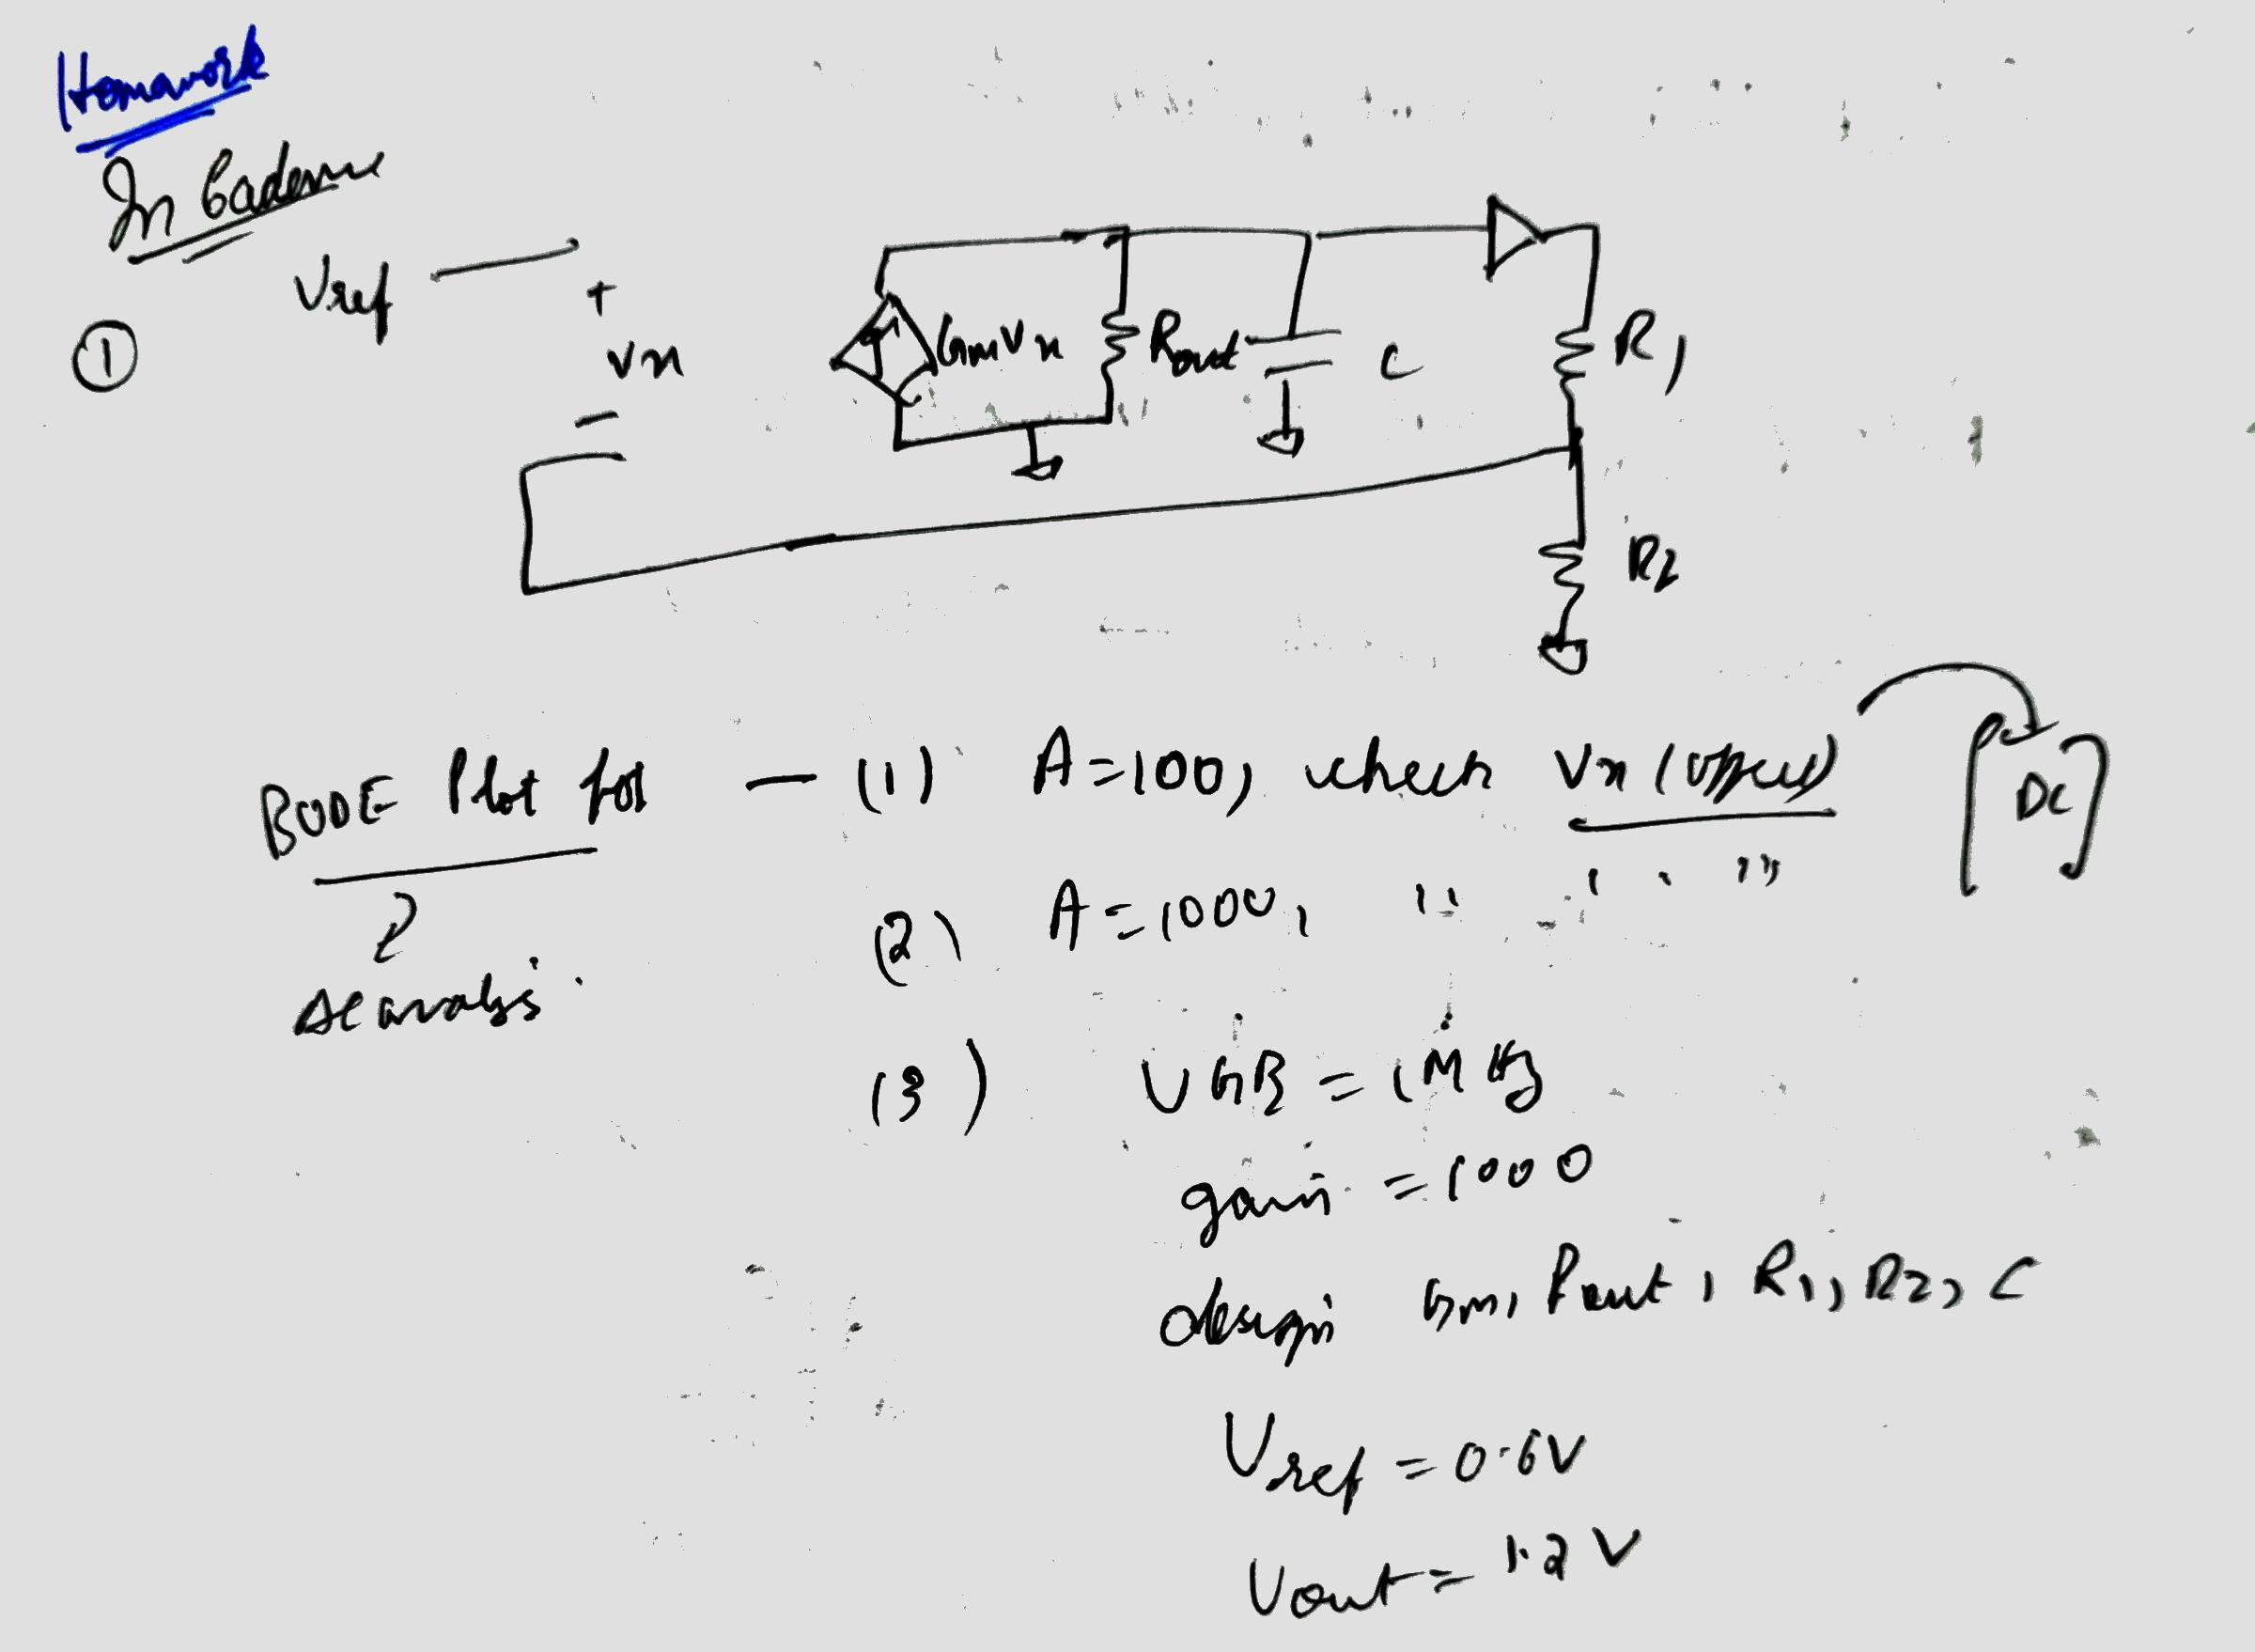
\includegraphics[width=0.8\linewidth]{images/Lec_5_Q_1.jpeg}
    \caption{Lecture 5 - Question 1}
\end{figure}
\subsection{Question 2}
In cadence, AC analysis. Bode Plot for $\frac{V_{out}}{V_{{in}}}$
\begin{enumerate}
    \item $G_{m_1} = G_{m_2} = 10 \mu F$ , $R_1 = R_2 = 10M \Omega$ , $C_1 = 10fF, C_2 = 2fF$
    \item add $C_{effective}$ at $C_1$ and get phase margin = $45^\circ$
\end{enumerate}
\begin{figure}
    \centering
    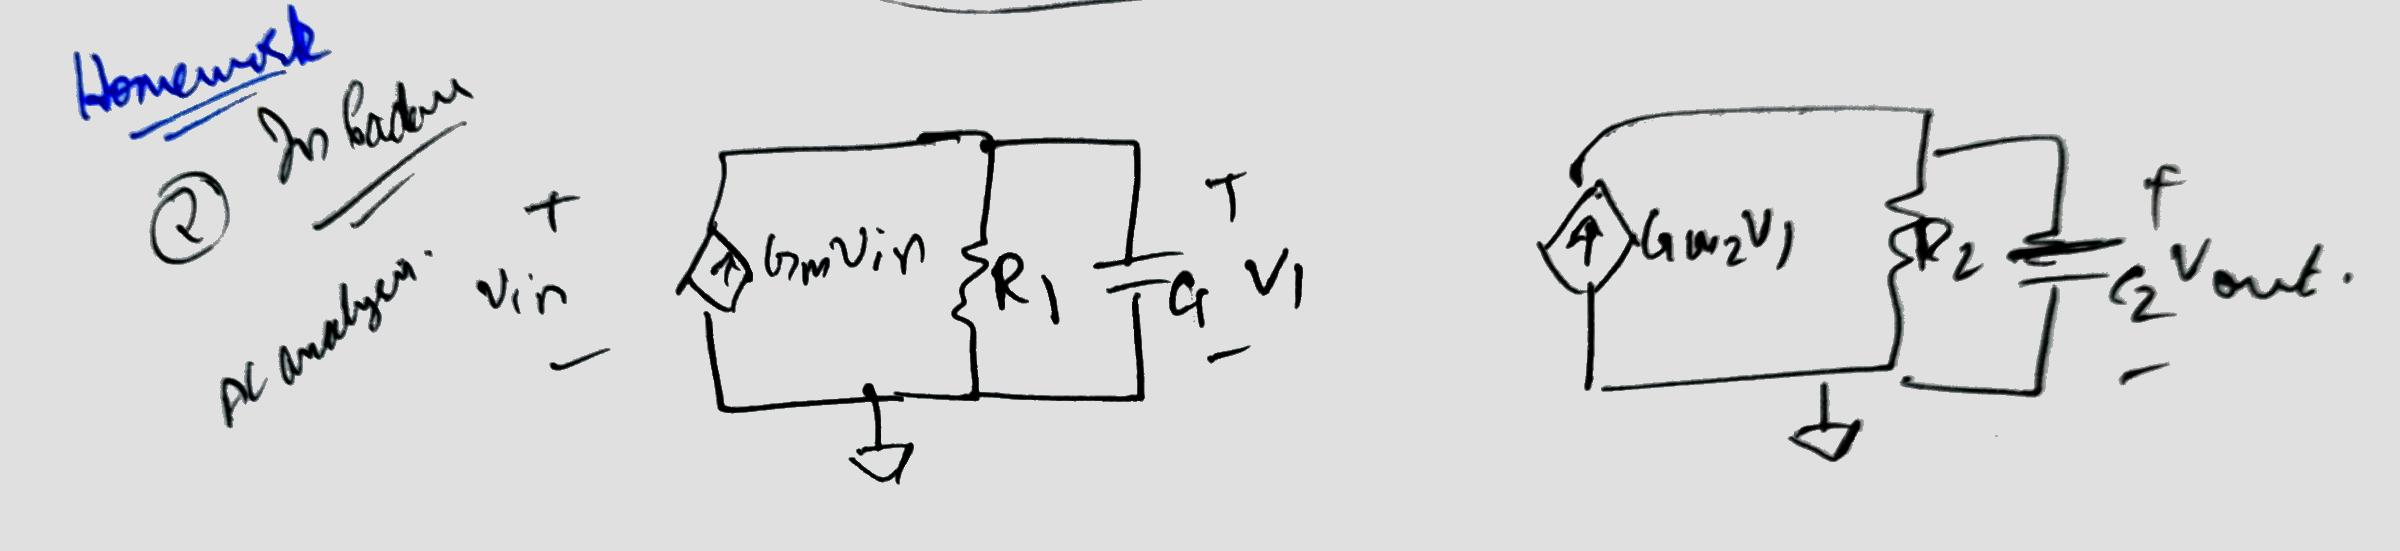
\includegraphics[width=0.8\linewidth]{images/Lec_5_Q_2_ckt.jpeg}
    \caption{Lecture 5 - Question 2 - circuit}
\end{figure}
\begin{figure}
    \centering
    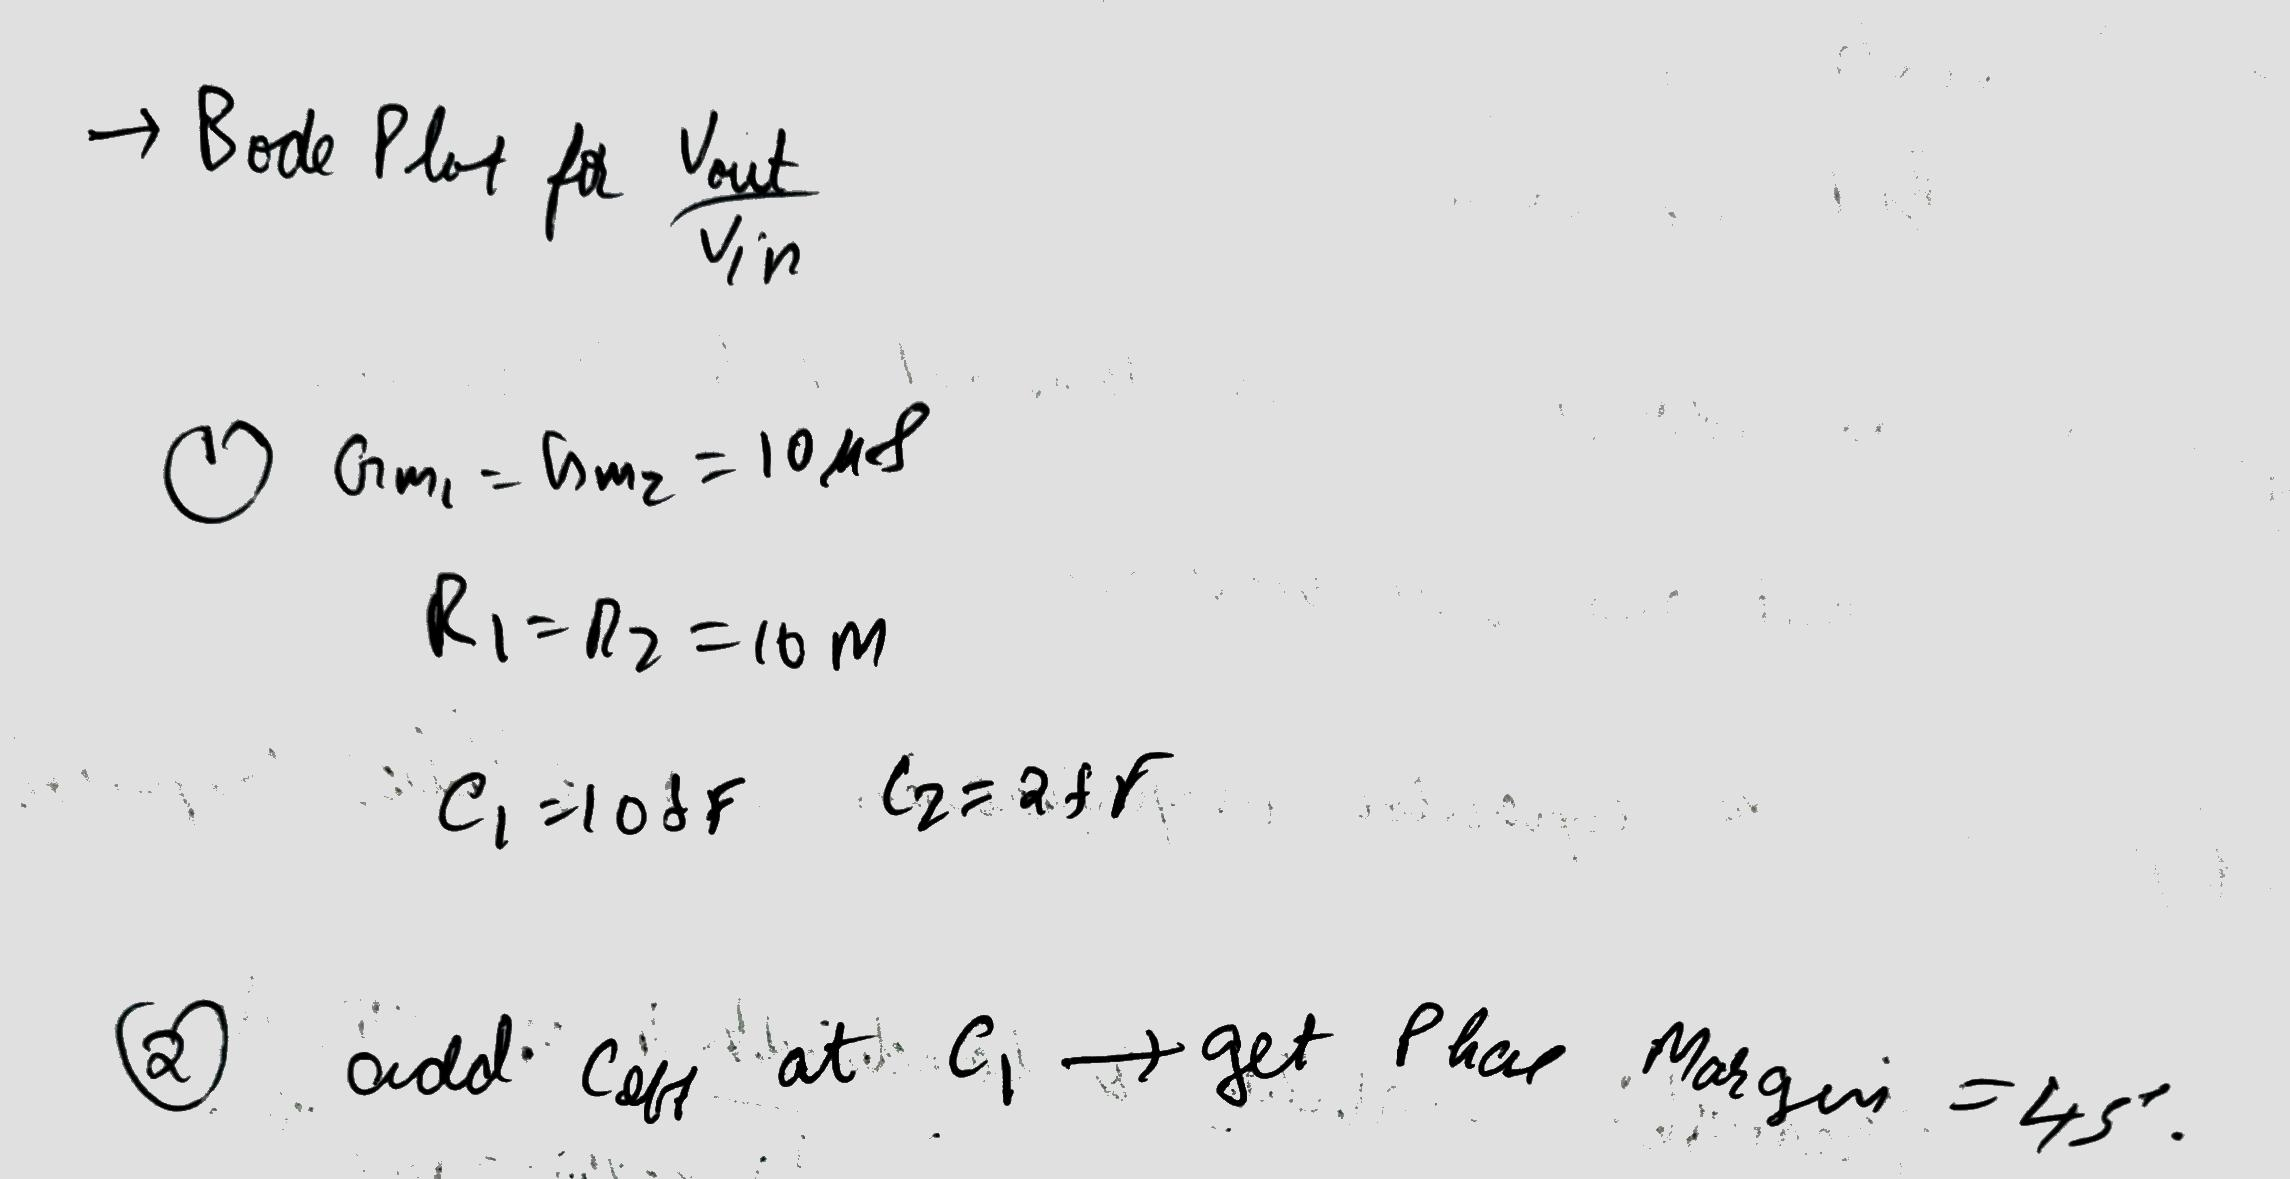
\includegraphics[width=1\linewidth]{images/Lec_5_Q_2_ques.jpeg}
    \caption{Lecture 5 - Question 2 - Question}
\end{figure}
\section{Lecture 6}
\subsection{Question 1}
Draw Bode plot for miller compensated circuit. \\ $G_{m_1} = G_{m_2} = 10 \mu S$ , $R_1 = R_2 = 10M \Omega$ , $C_1 = 10fF, C_2 = 2fF$ \\ Find Phase Margin, Unity Gain Bandwidth and DC Gain. (Theory + Cadence) (AC analysis/STB)
\begin{figure}
    \centering
    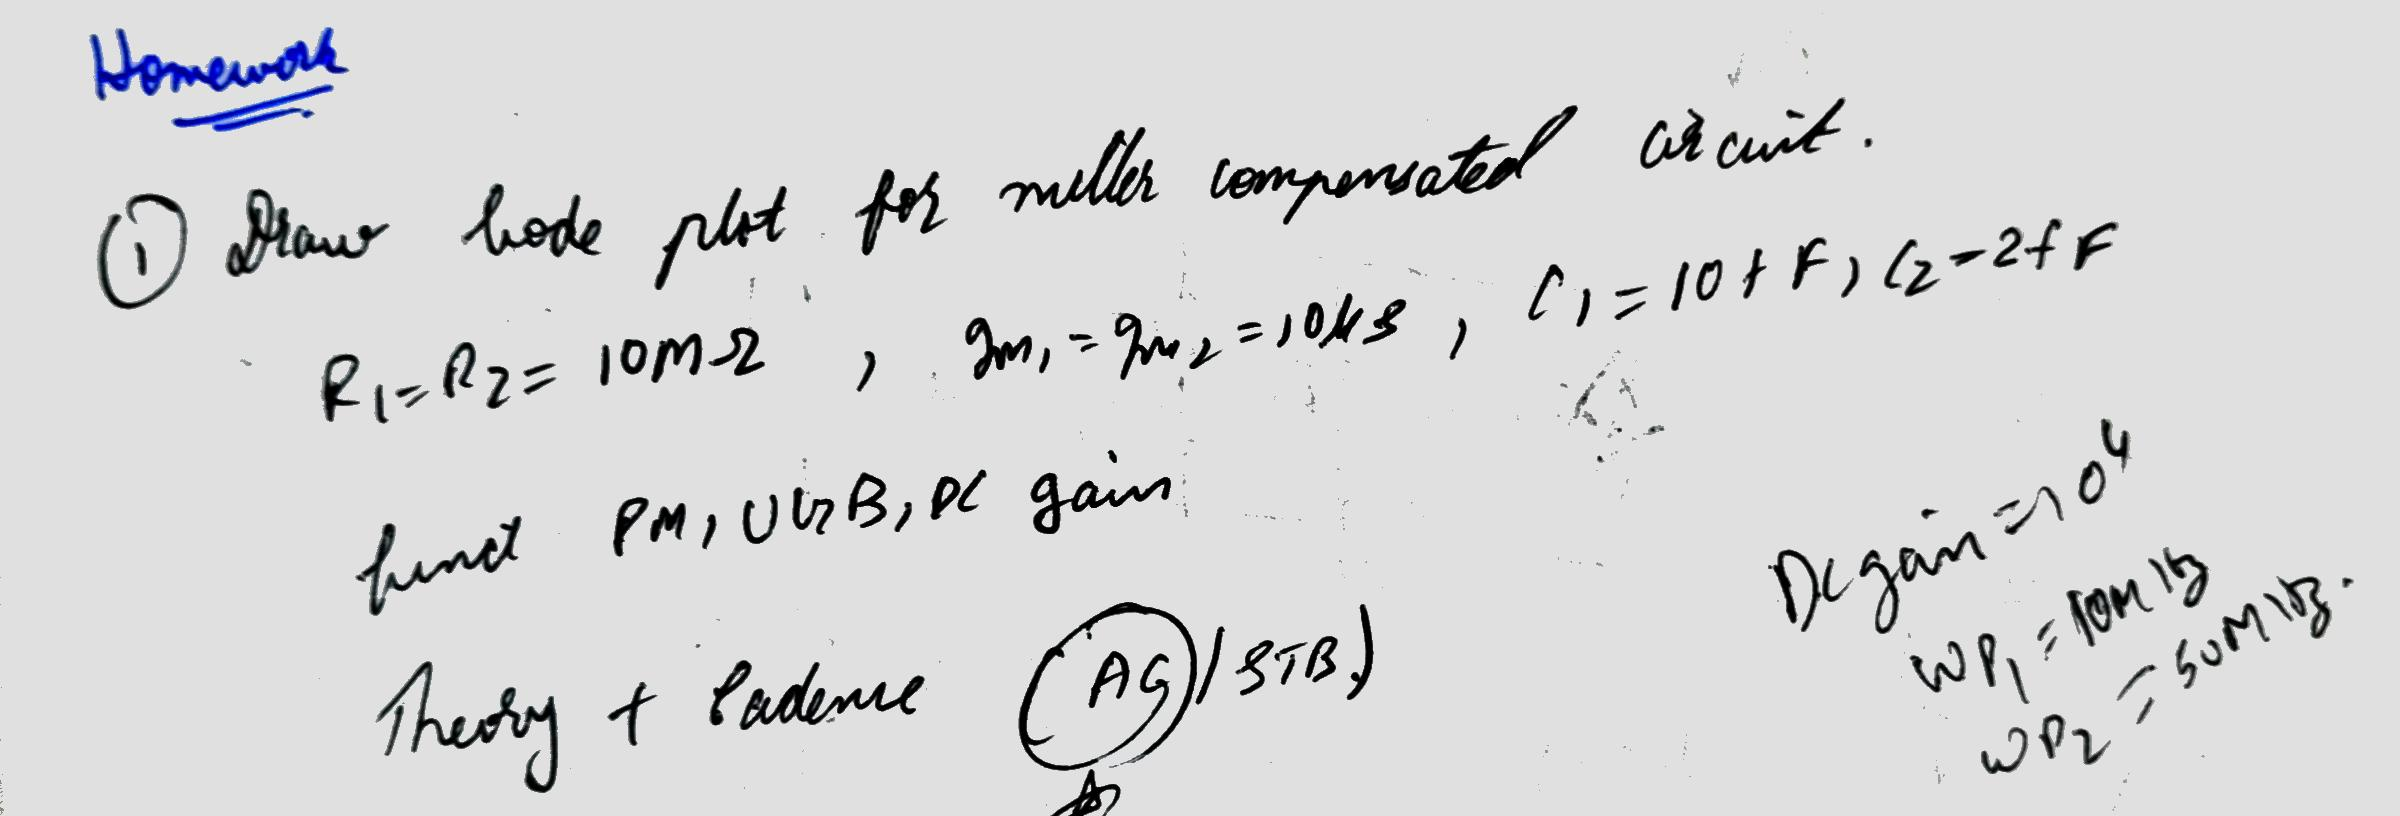
\includegraphics[width=0.8\linewidth]{images/Lec_6_Q_1.jpeg}
    \caption{Lecture 6 - Question 1}
\end{figure}
\subsection{Question 2}
Simulate in cadence.
\begin{figure}
    \centering
    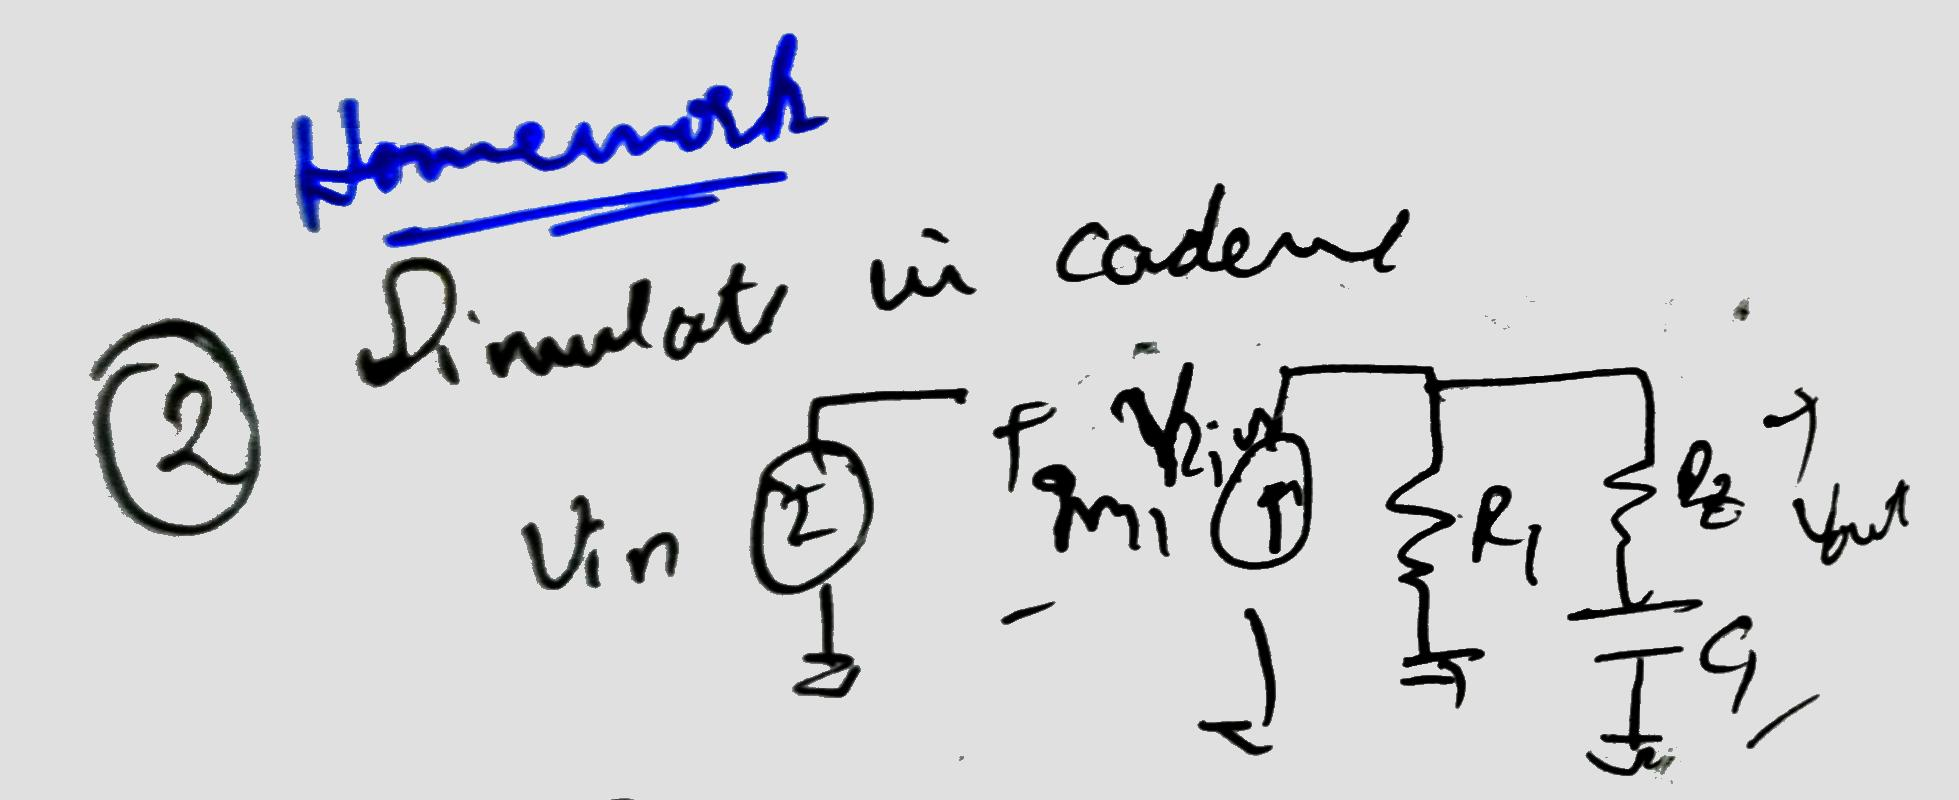
\includegraphics[width=0.8\linewidth]{images/Lec_6_Q_2.jpeg}
    \caption{Lecture 6 - Question 2}
\end{figure}
\section{Lecture 7}
\subsection{Question 1}
TSMC 18 lib, Simulate all the resistors $-40^\circ$ to $125^\circ$ (SS, TT, FF)
TSMC 18 lib, Simulate all the resistors $-40^\circ$ to $125^\circ$ (SS, TT, FF)
\begin{table}[ht]
\centering
\begin{tabular}{|l|l|l|l|l|l|}
\hline
Resistor & Temperature Coefficient & Type & Process Spread & Linearity & Area \\
\hline
R1 & Value & TypeA & Spread1 & Linear1 & Area1 \\
R2 & Value & TypeB & Spread2 & Linear2 & Area2 \\
R3 & Value & TypeC & Spread3 & Linear3 & Area3 \\
\hline
\end{tabular}
\caption{Resistor characteristics under different conditions}
\end{table}
\begin{figure}
    \centering
    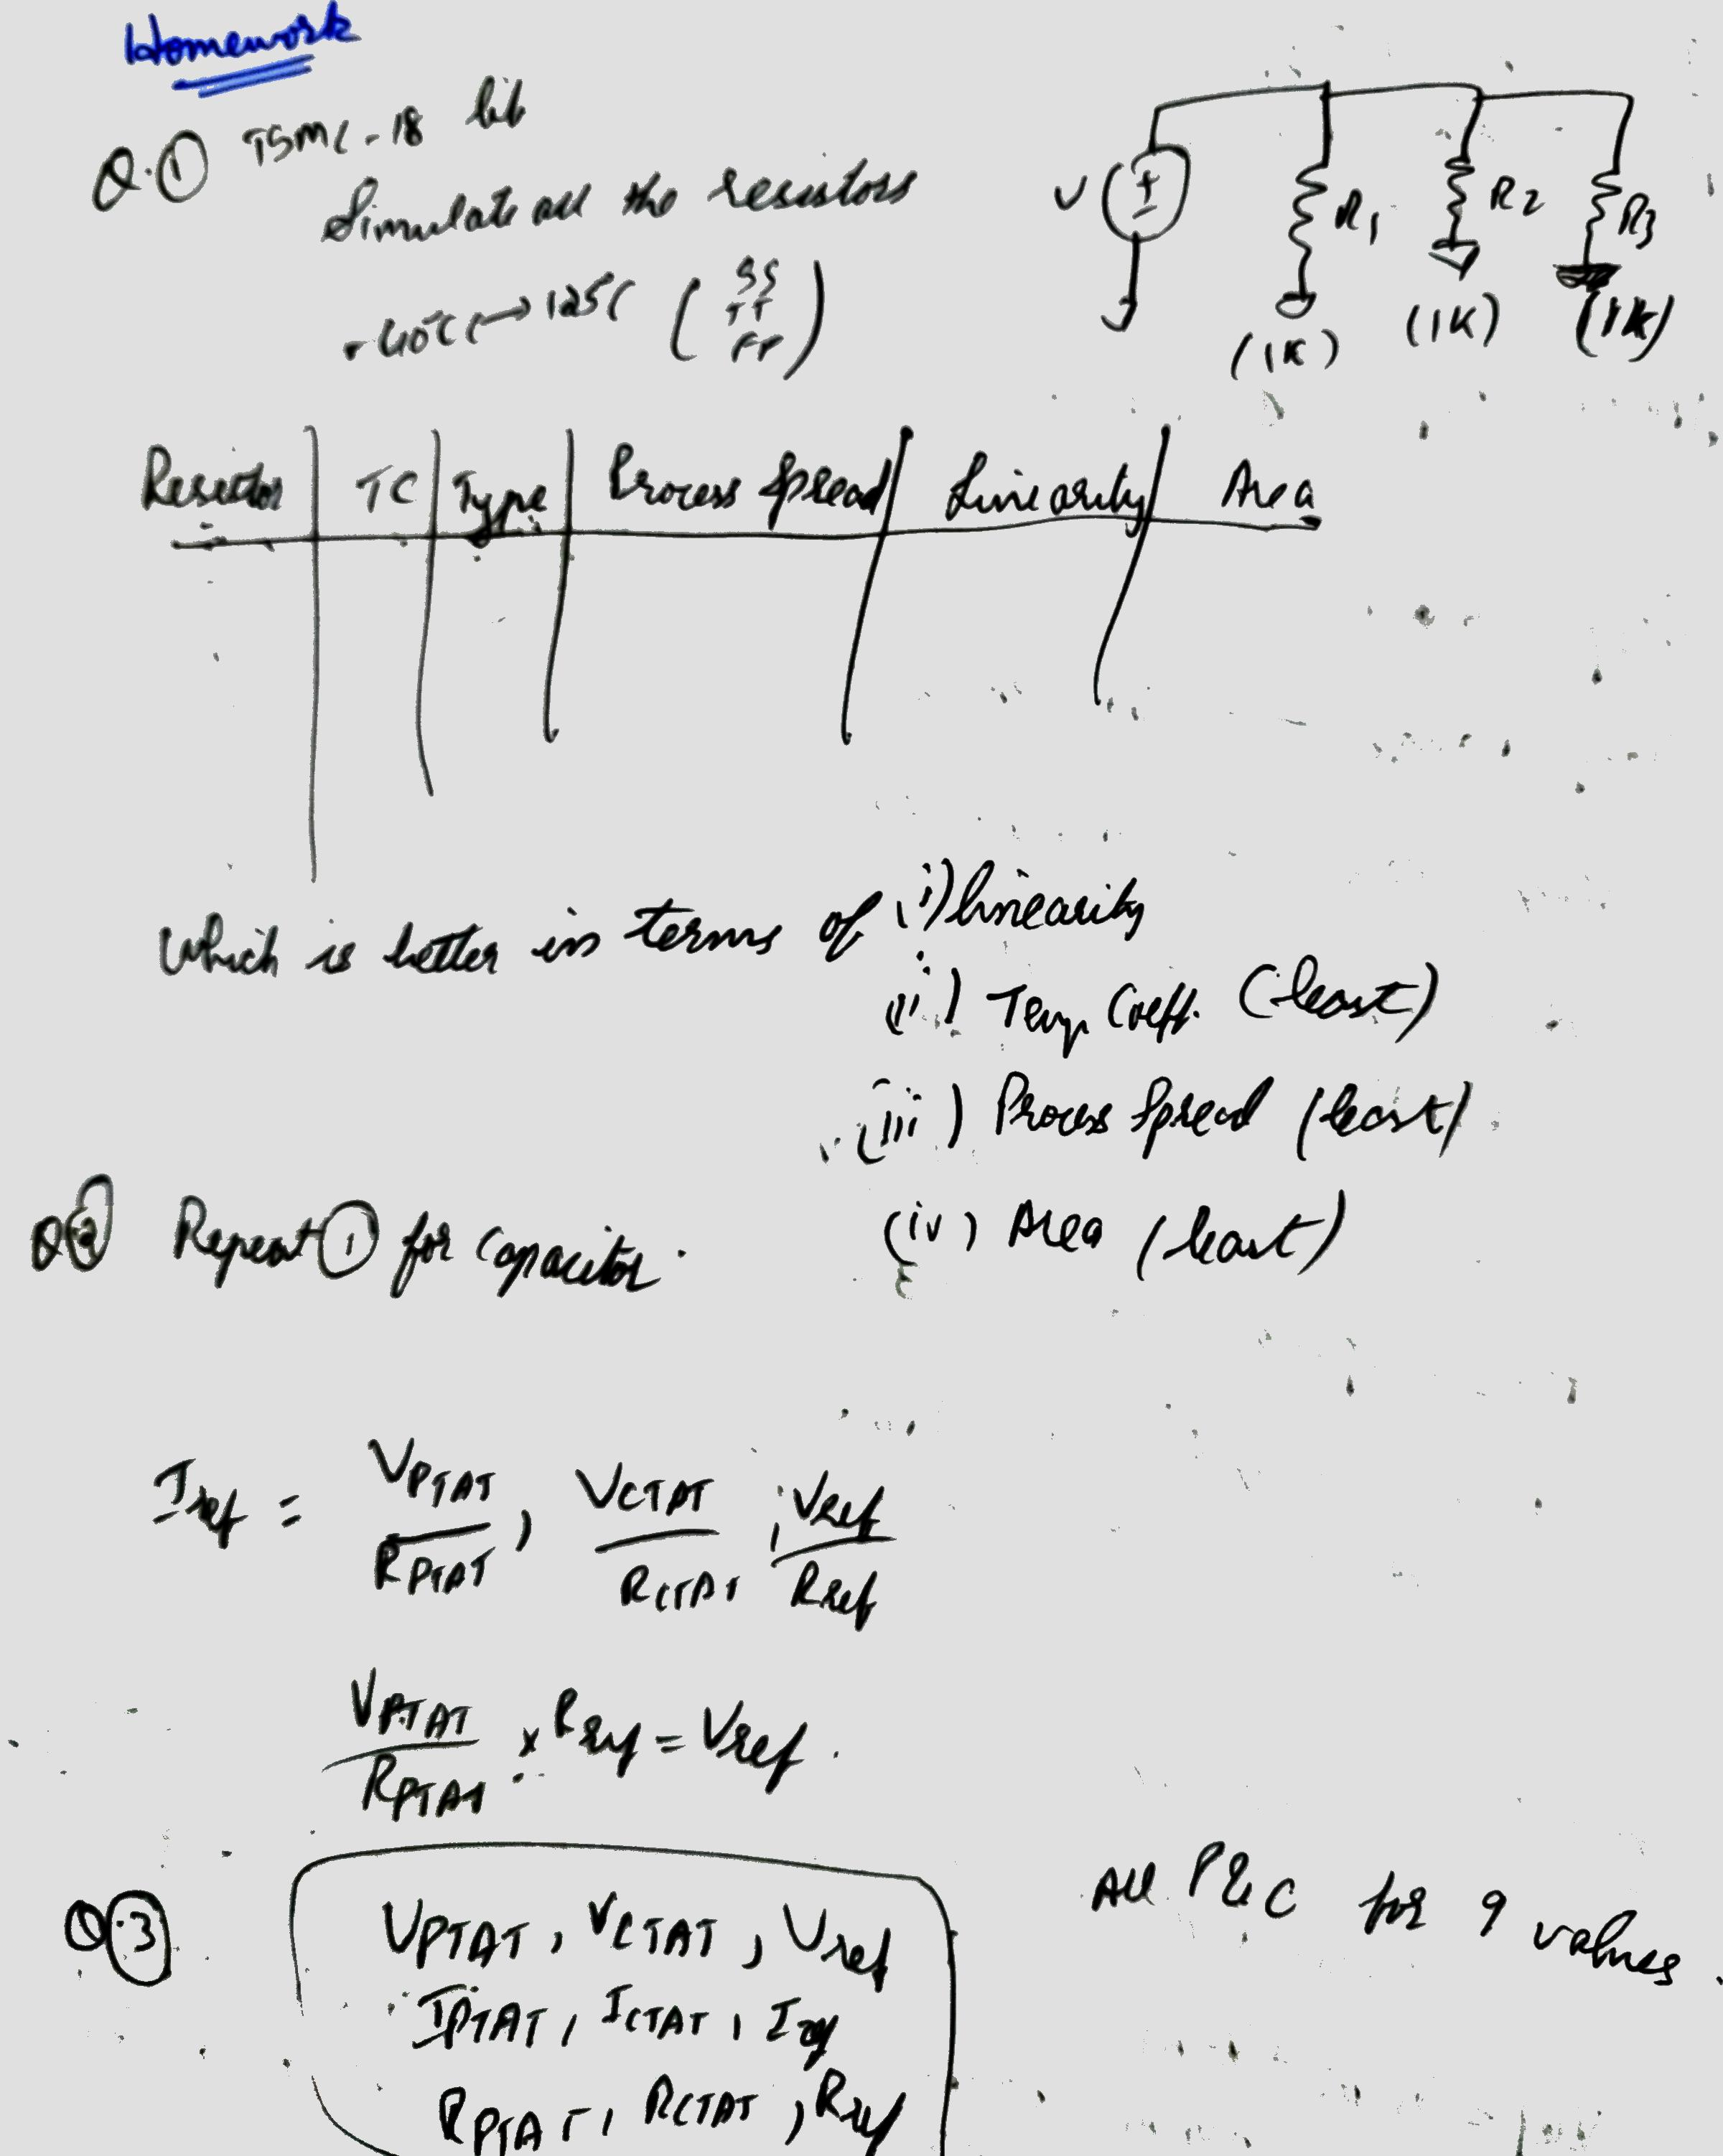
\includegraphics[width=0.8\linewidth]{images/Lec_7_Q_1_2_3.jpeg}
    \caption{Lecture 7 - Question 1,2,3}
\end{figure}
\subsection{Question 2}
Repeate Question 1 with a capacitor. 
\begin{table}[ht]
\centering
\begin{tabular}{|l|l|l|l|l|l|}
\hline
Capacitor & Temperature Coefficient & Type & Process Spread & Linearity & Area \\
\hline
C1 & Value & TypeA & Spread1 & Linear1 & Area1 \\
C2 & Value & TypeB & Spread2 & Linear2 & Area2 \\
C3 & Value & TypeC & Spread3 & Linear3 & Area3 \\
\hline
\end{tabular}
\caption{Resistor characteristics under different conditions}
\end{table}

\subsection{Question 3}
$V_{PTAT}, V_{CTAT}, V_{Ref}$\\ $I_{PTAT}, I_{CTAT}, I_{Ref}$\\ $R_{PTAT}, R_{CTAT}, R_{Ref}$\\
All P and C for 9 values.
% If you want to add a bibliography, include the following before \end{document}:
% \begin{thebibliography}{9}
% \bibitem{example} Author Name, \textit{Title of Paper}, Journal Name, Year.
% \end{thebibliography}

\end{document}